\documentclass[fontsize=11pt]{scrartcl}

\usepackage[ngerman]{babel}
\usepackage[utf8]{inputenc}
\usepackage[T1]{fontenc}
\usepackage{blindtext}
\usepackage{multicol}
\usepackage{url}
\usepackage{abstract}
\usepackage{graphicx}
\usepackage{amssymb}
\usepackage{amsmath}
\usepackage[]{algorithm2e}
\usepackage{caption}
\usepackage{wrapfig}
\usepackage{url}

\usepackage{lipsum}

\captionsetup{font=scriptsize}

%Eigene Bildumgebug definieren, weil das sonst seltsam ausgeht mit multicols
\newenvironment{Figure}
  {\par\medskip\noindent\minipage{\linewidth}}
  {\endminipage\par\medskip}

%Eigener Befehl um eine leere Seite einzufügen
\newcommand{\blankpage}{
\newpage
\thispagestyle{empty}
\mbox{}
\newpage
}

\newcommand*{\quelle}{% 
  \footnotesize Quelle: 
}

\newcommand*{\zitat}{%
    \footnotesize 
}

\clubpenalty10000
\widowpenalty10000
\displaywidowpenalty=10000

\author{Janek Boll}
\author{Steven Minich}
%\matrikelnummer{447344}
%\dozent{Prof. Dr. Andreas Rausch}
%\betreuer{Dirk Herrling, M.Sc.}
\date{\today}
%Einrücken der Zeile verhindern
\setlength{\parindent}{0em} 


\begin{document}
    %Titelseite hinzufügen
    \titlehead{%
 {\setlength{\unitlength}{1mm}
  \begin{picture}(0,0)
    \put(-19,4){
\includegraphics{tuclogo}}
    \put(132,-269){
\includegraphics{rechteck}}
  \end{picture}}
}

\begin{titlepage}
    \makeatletter
    \@titlehead

    \begin{center}
        \vskip25mm
        
        \hspace*{-40mm}{\makebox[140mm]{\Large Seminararbeit}}\par

        \vskip20mm

        \hspace*{-40mm}{\makebox[140mm]{\titlefont\huge Data Mining und Maschinelles Lernen}}

        \vskip5mm

        \hspace*{-40mm}{\makebox[140mm]{\titlefont\Large Basierend auf W. Ertels \glqq Grundkurs Künstliche Intelligenz\grqq}}\par
        %\vskip1mm
        %\hspace*{-40mm}{\makebox[140mm]{\titlefont\LARGE und Entwurf eines Geschäftsmodells}}\par


        \vskip20mm

        \hspace*{-40mm}{\makebox[140mm]{\LARGE Janek Boll}}\par
        \hspace*{-40mm}{\makebox[140mm]{\large Studiengang Informatik, 447344}}\par

        \vskip10mm

        \hspace*{-40mm}{\makebox[140mm]{\LARGE Steven Minich}}\par
        \hspace*{-40mm}{\makebox[140mm]{\large Studiengang Wirtschaftsinformatik, 446680}}\par

        \vskip10mm

        \hspace*{-40mm}{\makebox[140mm]{\Large \today}}\par

        \vskip60mm

        \hspace*{-40mm}{\makebox[140mm]{Institut für Informatik, TU Clausthal}}\par

        \hspace*{-40mm}{\makebox[140mm]{Prof. Dr. Jörg P. Müller}}\par

        %\vskip08mm
        
        %\hspace*{-40mm}{\makebox[140mm]{betreut durch:}}\par

        %\hspace*{-40mm}{\makebox[140mm]{Dirk Herrling, M. Sc.}}\par


    \end{center}
\end{titlepage}

    %Leere Seite, weil sonst die Erklärung auf der Rückseite des Deckblatts wäre
    \blankpage

    %Eidesstattliche Erklärung
    \makeatletter

\cleardoublepage

\thispagestyle{empty}
\hskip 0mm
\vfill

\begin{center}
    \sffamily\bfseries\large Eidestattliche Erklärung
\end{center}

\bigskip\noindent Hiermit erkläre ich an Eides statt, dass ich die vorliegende Arbeit selbstständig verfasst und keine anderen als die angegebenen Hilfsmittel verwendet habe.\par
Mit einer Veröffentlichung der Arbeit in der Instituts- beziehungsweise Universitätsbibliothek bin ich einverstanden.\par

\bigskip\noindent Clausthal-Zellerfeld,~ \today\par
\vskip 10mm
\hfill \hrulefill\par
\hfill Janek Boll
\makeatother
    \newpage
    \makeatletter

\cleardoublepage

\thispagestyle{empty}
\hskip 0mm
\vfill

\begin{center}
    \sffamily\bfseries\large Eidestattliche Erklärung
\end{center}

\bigskip\noindent Hiermit erkläre ich an Eides statt, dass ich die vorliegende Arbeit selbstständig verfasst und keine anderen als die angegebenen Hilfsmittel verwendet habe.\par
Mit einer Veröffentlichung der Arbeit in der Instituts- beziehungsweise Universitätsbibliothek bin ich einverstanden.\par

\bigskip\noindent Osterode,~ \today\par
\vskip 10mm
\hfill \hrulefill\par
\hfill Steven Minich
\makeatother

    \blankpage
    
    % Abstract zentrieren
    \topskip0pt
    \vspace*{\fill}
    
    % Abstract
    \begin{abstract}
        \emph{Maschinelles Lernen} stellt einen sich schnell entwickelnden Teilbereich der \emph{künstlichen Intelligenz} dar. Durch erhöhte Rechenleistung und Speicherkapazität sind die verwendeten Verfahren auf immer größeren Datenmengen effektiv anwendbar. Daher ist es wenig verwunderlich, dass ein wichtiges Anwendungsgebiet für \emph{maschinelles Lernen} das \emph{Data Mining}, das heißt das Extrahieren von Wissen aus großen Datenmengen, ist. In dieser Arbeit sollen die notwendigen Grundlagen der Statistik sowie des Lernens mit Lehrer dargestellt werden.
    \end{abstract}
    \vspace*{\fill}
    
    \newpage
    
    %Inhaltsverzeichnis
    \tableofcontents
    
    \newpage

    %\begin{multicols}{2}
        \section{Einleitung}

            Als \emph{Data Mining} werden Verfahren bezeichnet, deren Ziel es ist, Wissen aus großen Datenmengen zu extrahieren. Dazu werden Verfahren aus der \emph{Statistik} und des \emph{maschinellen Lernens} eingesetzt.\cite{ertel2016}
            \emph{Maschinelles Lernen} ist ein Teilbereich der \emph{Künstlichen Intelligenz}, dessen Aufgabe das Lernen von Abbildungen einer Eingabemenge in eine Ausgabemenge ist. Typische Anwendungen sind die \emph{Klassifikation}, also eine Abbildung einer Eingabe auf eine Klasse, und \emph{Approximation}, sprich die Berechnung eines Funktionswertes, der möglichst nahe an der Realität ist.\cite{ertel2016,mlfor}
            In den vergangenen Jahren hat das \emph{maschinelle Lernen} große Fortschritte gemacht, was im Wesentlichen auf die Zunahme von Rechenleistung und Speicherkapazität zurückgeführt werden kann.\cite{mlfor}
            So werden bereits heute medizinische Diagnosen unter Verwendung sogenannter \emph{Expertensysteme} gestellt\cite{ertel2016} und Behandlungspläne für Krebspatienten durch maschinelles Lernen unter Verwendung der Patientendaten anderer Patienten automatisch erstellt.\cite{mlfor}
            Der Online-Versandhändler Amazon setzt Data Minig ein, um seinen Kunden relevante Artikel zu präsentieren.\cite{ertel2016}
            Auch bei der Kreditvergabe setzen Finazdienstleister heutzutage maschinelle Lernverfahren ein, um Kreditanfragen zu prüfen.\cite{mlfor}
            Mit zunehmender Bedeutung von \emph{Data Mining} und \emph{maschinellem Lernen} sind auch leicht zu verwendende Frameworks erschienen, die dem Anwender einen leichten Einstieg in die Materie ermöglichen. Zu den bekanntesten Vertretern gehören \emph{Scikit Learn}\footnote{\url{https://scikit-learn.org/stable/}}, ein Framework für die Programmiersprache Python, und \emph{Tensorflow}\footnote{\url{https://www.tensorflow.org}}, ein Framework von Google.
            Da künstliche Intelligenz und insbesondere maschinelles Lernen bereits Einfluss auf das tägliche Leben haben, und davon auszugehen ist, dass dieser Einfluss in den kommenden Jahren weiter zunimmt, soll im Rahmen dieser Arbeit ein grundlegendes Verständnis für die zugrundeliegenden Verfahren hergestellt werden. Wir werden uns dabei auf statistische Lage-, Streuungs- und Zusammenhangsmaße im Bereich der Statistik und auf Lernverfahren mit Lehrer im Bereich des maschinellen Lernens konzentrieren.

        \section{Statistische Grundlagen}
            
            \subsection{Skalenniveaus}
                Untersuchte Merkmale können unterschiedliche Eigenschaften bezüglich ihrer Messbarkeit aufweisen. Diese Eigenschaften haben wesentlichen Einfluss darauf, welche Lage-, Streuungs- und und Zusammenhangsmaße auf diese Merkmale angewendet werden können.
                Daher sollen im Folgenden zunächst \emph{Skalenniveaus} eingeführt werden, anhand welcher die Unterschiede der verschiedenen Messbarkeitseigenschaften deutlich werden.
                % Untersuchte Merkmale können anhand ihrer Messbarkeitseigenschaften unterschieden und in die Kategorien \emph{qualitative}, \emph{komparative} und \emph{quantitative Merkmale} eingeteilt werden.
                % Qualitative Merkmale sind solche, deren Ausprägungen sich in ihrer Art unterscheiden. 
                % \cite{kohn2005}
            \subsection{Nominalskala}
                Die einfachste Skalierung in der deskriptiven Statistik ist die sogenannte \emph{Nominalskala}. Die untersuchten Merkmale lassen sich nur im Hinblick auf Gleich- beziehungsweise Ungleichheit untersuchen; eine Ordnung der Merkmalsausprägungen ist nicht möglich. 
                \cite{kohn2005}
                \subsubsection{Beispiel}
                    An einer Kreuzung werden die vorbeifahrenden Autos hinsichtlich ihrer Farbe untersucht. Mögliche Ausprägungen des untersuchten Merkmals Farbe sind etwa \emph{Grün}, \emph{Schwarz}, \emph{Weiß}, \emph{Gelb} und \emph{Rot}. Zwar lassen sich die Merkmalsausprägungen voneinander unterscheiden, aber offensichtlich ist ein rotes Auto nicht besser oder schlechter als ein gelbes oder schwarzes Auto.
                \subsection{Ordinalskala}
                    Ordinalskalierte Merkmale sind solche, bei denen neben der Unterscheidbarkeit der Merkmalsausprägungen auch eine natürliche Reihenfolge der Ausprägungen zugrunde liegt, wobei der Abstand zwischen den einzelnen Merkmalsausprägungen aber nicht sinnvoll interpretierbar ist. \cite{kohn2005}
                    \subsubsection{Beispiel}
                        Die gängigen Kleidergrößen von XS bis XXL verdeutlichen dies. Offenbar ist eine Größe M größer als eine Größe XS, jedoch ist keine Aussage über das Verhältnis des Größenunterschieds der beiden Größen möglich.
                \subsection{Metrische Skalen}
                    Eine Skala, deren Merkmalsausprägungen reelle Zahlen sind, und die auch die Ordnungsstruktur der reellen Zahlen aufweist, wird \emph{metrische Skala} genannt. Neben der Unterscheidung verschiedener Merkmalsausprägungen und der zugrunde liegenden Ordnungsrelation zeichnen sich metrische Zahlen dadurch aus, dass die Merkmalsausprägungen jeden möglichen Wert annehmen können. Da die Werte reelle Zahlen sind gibt es also überabzählbar unendlich viele Merkmalsausprägungen und der Wertebereich metrischer Skalen wird \emph{stetig} genannt. Neben der Stetigkeit des Wertebeichs ist die Möglichkeit der sinnvollen Interpretation der Abstände von metrisch skalierten Merkmalen eine charakterisierende Eigenschaft ebendieser.
                    \cite{kohn2005}
                    \subsubsection{Beispiel}
                        Die Entfernung zweier Punkte in Metern weist die Eigenschaften metrisch skalierter Merkmale auf: Zum einen kann die Entfernung zweier Punkte jeden beliebigen reellen Wert annehmen, zum anderen lassen sich verschiedene Merkmalsausprägungen problemlos ordnen; eine Entfernung von $ 0,5m $ ist kleiner als eine Entfernung von $ 0,78m $. Darüber hinaus ist auch der Abstand interpretierbar, so ist ein Abstand von $4m$ augenscheinlich viermal so groß wie ein Abstand von $1m$.
                    \subsubsection{Weitere Unterscheidung metrischer Merkmale}
                        Anhand der Existenz eines natürlichen Nullpunktes lassen sich metrisch skalierte Merkmale weiter unterscheiden. Ein metrisches Merkmal heißt \emph{intervallskaliert}, wenn es keinen natürlichen Nullpunkt gibt. \cite{kohn2005} Ein Beispiel hierfür ist die Temperatur, der Nullpunkt ist willkürlich festgesetz. Misst man die Temperatur in Grad Celsius, so entspricht der Nullpunkt dem Gefrierpunkt von Wasser, misst man jedoch in Grad Fahrenheit, so entspricht der Gefriepunkt von Wasser $32$ Grad Fahrenheit und der Nullpunkt in Grad Fahrenheit entspricht etwa $-17,78$ Grad Celsius.
                        \newline
                        Exsitiert hingegen ein natürlicher Nullpunkt, so spricht man von \emph{verhältnisskalierten} Merkmalen. \cite{kohn2005}
                        \newline
                        Ein Beispiel für ein verhältnisskaliertes Merkmal stellt das Gewicht dar. Zwar existieren verschiedene Maßeinheiten wie Gramm, Pfund oder Unzen, jedoch entspricht ein Gewicht von $0$ Gramm ebenso einem Gewicht von $0$ Pfund und ebenso $0$ Unzen.
                
                \subsection{Lagemaße}
                    Einen ersten Ansatz zur Datenanalyse liefern sogenannte \emph{Lagemaße}. Sie liefern Aufschluss über die Häufigkeitsverteilung der untersuchten Merkmale einer Stichprobe. \cite{kohn2005}
                    
                    \subsubsection{Modus}
                        Der \emph{Modus} $x_{mod}$ ist ein sehr einfaches Lagemaß, das sich hauptsächlich für nominalskalierte Merkmale eignet. Der Modus ist die Merkmalsausprägung mit der größten Häufigkeit.\cite{kohn2005}
                    
                        \subsubsection{Median}
                        Der \emph{Median} $x_{med}$ entspricht dem Wert in der Mitte. Es folgt, dass der Median nur für mindestens ordinalskalierte Merkmale angewendet werden kann, da den Merkmalsausprägungen eine Ordnungsstruktur zugrundeliegen muss.\cite{kohn2005}
                        \newline
                        Zur Berechnung des Medians wird wie folgt vorgegangen: Zuächst werden die Merkmalsausprägungen geordnet und anschließend das mittlere Element ausgewählt. Seien dazu $n$ Stichproben genommen worden und es entspreche $x_i,i \in \{1,\dots,n\}$ dem Wert der $i$-ten Probe. Analog entspreche $x_{(i)}, i \in \{1,\dots,n\}$ der geordneten Probe, d.h. $x_{(i)} \leq x_{(i+1)} \forall i \in \{1,\dots,n\}$.
                        \newline
                        Zur Bestimmung des mittleren Elements der Probe muss unterschieden werden, ob die Probe aus einer geraden oder ungeraden Anzahl von Elementen besteht, das heißt, ist $n$ gerade oder ungerade.
                        \newline
                        $$
                            x_{med}:=\left\{\begin{array}{cl} x_{(\frac{n+1}{2})}, & \mbox{falls n ungerade }\\ \frac{1}{2}\left( x_{(\frac{n}{2})} + x_{(\frac{n}{2}+1)} \right), & \mbox{sonst} \end{array}\right. \text{ \footnotesize\cite[S.12]{ingstat}}
                        $$
                        % Fall 1 \cite{ertel2016}:
                        % \newline
                        % $n$ ungerade
                        % $$ 
                        % x_{med} := x_{(\frac{n+1}{2})}
                        % $$
                        % Fall 2\cite{ertel2016}:
                        % \newline
                        % $n$ gerade
                        % $$ 
                        %     x_{med} := \frac{1}{2}\left( x_{(\frac{n}{2})} + x_{(\frac{n}{2}+1)} \right)
                        % $$
                    
                        \subsubsection{Arithmetisches Mittel}
                        Das \emph{arithmetische Mittel} stellt das am weitesten verbreitette Lagemaß für metrische Merkmale dar. Im Gegensatz zu Modus und Median berücksichtigt das arithmetische Mittel alle Merkmalsausprägungen einer Probe, wird dadurch aber auch anfällig für \emph{Ausreißer}.
                        $$ 
                            \bar{x} := \frac{1}{n}\sum_{i=1}^nx_i \text{ \footnotesize\cite[S.11]{ingstat}}
                        $$
                        Aus der Formel folgt direkt, dass das arithmetische Mittel nicht auf nominal- oder ordinalskalierte Merkmale angewendet werden kann, da auf diesen keine Addition definiert ist.

                \subsection{Streuungsmaße}
                    Streuungsmaße geben Auskunft darüber, wie stark die Ausprägungen des untersuchten Merkmals von einem Lagemaß, wie dem arithmetischen Mittel, abweichen, also wie sehr sie um den Mittelwert streuen. Sie liefern damit eine Beurteilungsmöglichkeit für das verwendete Lagemaß.\cite{ertel2016,kohn2005}
                    
                    \subsubsection{Varianz}
                        Die \emph{Varianz} $\sigma^2$ ist das am häufigsten verwendete Streuungsmaß. Sie beschreibt die \emph{mittlere quadratische Abweichung} der Merkmalsausprägungen vom Mittelwert.
                        Wird die Grundgesamtheit betrachtet, so gilt die folgende Formel (\emph{empirische Varianz}): 
                        $$
                            \sigma^2 := \frac{1}{n}\sum_{i=1}^n(x_i - \bar{x})^2 \text{ \footnotesize\cite[S.74]{kohn2005}}
                        $$
                        Soll dagegen lediglich eine Stichprobe, das heißt eine Teilmenge der Grundgesamtheit, untersucht werden, so muss die Formel angepasst werden (\emph{Stichprobenvarianz}):
                        $$
                            \sigma^2 := \frac{1}{n-1}\sum_{i=1}^n(x_i - \bar{x})^2 \text{ \footnotesize\cite[vgl. S. 74]{kohn2005}}
                        $$
                        In beiden Fällen ist jedoch zu beachten, dass die Maßeinheit der Varianz, aufgrund der Quadrierung des Abstandes zum Mittelwert, nicht mehr der Maßeinheit der urspürnglichen Werte entspricht.\cite{kohn2005}
                    
                    \subsubsection{Standardabweichung}
                        Die \emph{Standardabweichung} $\sigma$ ist die positive Quadratwurzel der Varianz. Wie bereits erläutert entspricht die Maßeinheit der Varianz nicht der ursprünglichen Maßeinheit der Werte. Dieses Manko lässt sich mit der Standardabweichung beheben.
                        $$ \sigma := + \sqrt{\sigma^2} \text{ \footnotesize\cite[S.76]{kohn2005}}$$
                        Durch das Ziehen der Quadratwurzel misst die Standardabweichung die mittlere Streuung um den Mittelwert in der gleichen Maßeinheit wie die ursprünglichen Werte.\cite{kohn2005}

                \subsection{Zusammenhangsmaße}
                    Häufig, so auch im Bereich des \emph{Data Mining}, interessiert man sich jedoch nicht nur für die Ausprägungen eines einzelnen Merkmals. Viel interessanter erscheint eine Untersuchung wie verschiedene Merkmale zueinander in Beziehung stehen. Unter Umständen lassen sich aus den Beobachtungen eines Merkmals Rückschlüsse auf ein anderes Merkmal ziehen.
                    
                    \subsubsection{Kovarianz}
                        Die \emph{Kovarianz} $cov(x,y)$ beschreibt, wie sich zwei Merkmale eines beobachteten Merkmalsvektors zueinander in Bezug auf Abweichung ihres jeweiligen Mittelwerts verhalten.\cite{ertel2016}\\
                        Definition der Kovarianz:\\
                        Seien $x,y$ zwei Merkmale eines Merkmalsvektors, $n$ die Anzahl der in einer Stichprobe untersuchten Merkmalsvektoren. Dann gilt für die Kovarianz:
                        $$
                            cov(x,y) := \frac{1}{n-1}\sum_{i=1}^n(x_i - \bar{x})(y_i - \bar{y}) \text{ \footnotesize\cite[S.121]{kohn2005}}
                        $$
                        Aus der Definition folgt unmittelbar, dass der $i$. Merkmalsvektor einen positiven Beitrag zur Summe liefert, wenn die Merkmale $x$ und $y$ in die gleiche Richtung vom Mittelwert abweichen. Analog liefert eine Abweichung der Merkmale in unterschiedliche Richtung vom Mittelwert einen negativen Beitrag zur Summe. \cite{ertel2016}

                    \subsubsection{Korrelationskoeffizient}
                        Da der Wert der Kovarianz unter anderem auch von den Absolutwerten der Variablen abhängt, ist ein Vergleich der Werte problematisch.
                        \cite{ertel2016} \\
                        Um diese Abhängikeit von den Absolutwerten zu eliminieren wird der \emph{Korrelationskoeffizient $\rho_{xy}$} als normierte Kovarianz definiert als Kovarianz der beiden Variablen geteilt durch das Produkt der Standardabweichung von $x$ und $y$:
                        $$
                            \rho_{xy} := \frac{cov(x,y)}{\sigma_x \cdot \sigma_y} \text{ \footnotesize\cite[S.122]{kohn2005}}
                        $$
                        Der Korrelationskoeffizient ist normiert auf das Intervall $[-1,1]$, das heißt es gilt $-1 \leq K_{xy} \leq 1)$
                        \cite{kohn2005}

        \section{Maschinelles Lernen}
            
            \subsection{Lernen mit und ohne Lehrer}
                Eine erste Einteilung verschiedener maschineller Lernverfahren ist die, ob das Lernverfahren auf Trainingsdaten, also auf solche Daten, für die eine korrekte Klasseneinordnung oder Funktionswert bereits bekannt ist, verwenden. In diesem Fall wird von \emph{Lernen mit Lehrer} oder \emph{supervised learning} gesprochen. Die richtige Klassifikation wird häufig von \emph{Experten} vorgenommen.\cite{ertel2016}
                \\
                Lernverfahren, die hingegen \emph{ohne} Trainingsdaten auskommen, werden als Verfahren aus dem Bereich \emph{Lernen ohne Lehrer} (\emph{unsupervised learning}) bezeichnet.\\
                In dieser Arbeit beschränken wir uns ausschließlich auf Lernverfahren, die auf der Verwendung von Trainingsdaten beruhen, bleiben also im Bereich des \emph{Lernens mit Lehrer}.

            \subsection{Agenten}
                Der Begriff des \emph{Agenten} ist in vielen Teilbereichen der Informatik von zentraler Bedeutung, allerdings wird der Agentenbegriff in verschiedenen Teilbereichen unterschiedlich ausgelegt. So stellt ein Agent in der klassischen Informatik eine Abbildung von einer Eingabe auf eine Ausgabe dar und wird als \emph{Software-Agent} bezeichnet, während ein Agent in der Robotik einen \emph{Hardware-Agenten} bezeichnet, der eine Erweiterung des Software-Agenten um Sensoren und Aktoren darstellt, die es dem Hardware-Agenten ermöglichen, seine Umgebung wahrzunehmen und zu verändern.\cite{ertel2016}
                \begin{Figure}
                    \centering
                    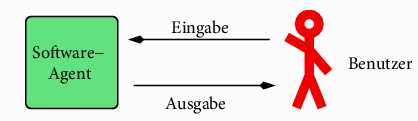
\includegraphics[scale=0.6]{softwareagent.png}
                    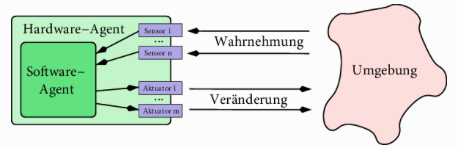
\includegraphics[scale=0.6]{hardwareagent.png}
                    \captionof{figure}{
                        Soft- und Hardware-Agent
                    }
                    \raggedleft \footnotesize\cite[S.18, Abb. 1.5, S19, Abb. 1.6]{ertel2016}
                    % \quelle W. Ertel, Grundkurs künstliche Intelligenz, Springer Fachmedien, S. 18, Abb. 1.5 und S. 19 Abb. 1.6
                \end{Figure}
                Auch bezüglich ihrer Intelligenz unterscheiden sich Agenten voneinander.
                Ein Agent, der lediglich eine Abbildung von der Menge aller möglichen Eingaben auf die Menge aller möglichen Ausgaben implementiert, wird als \emph{Reflex-Agent} bezeichnet. Ein Reflex-Agent ist in der Lage, Probleme zu lösen, bei denen es sich um Markov-Entscheidungsprozesse handelt. Zur optimalen Lösung dieser Klasse von Problemen ist lediglich Wissen über den aktuellen Zustand der Umgebung erforderlich.\cite{ertel2016}
                \newline
                \emph{Agenten mit Gedächtnis} hingegen sind Agenten, die bei ihren Entscheidungen Wissen über vorangegange Zustände der Umgebung berücksichtigen können.\cite{ertel2016}
            
            \subsubsection{Der lernende Agent}
            \label{subsec:lernenderagent}
                Der im Rahmen dieser Arbeit zentrale Agentenbegriff ist der des \emph{lernenden Agenten}. Der lernende Agent entspricht einer Abbildung eines Eingabevektors auf eine diskrete Klasse oder einen stetigen Funktionswert. Er unterscheidet sich vom Reflex-Agenten dadurch, dass die konkrete Abbildungsvorschrift nicht vom Programmierer vorgegeben, sondern aus \emph{Trainingsdaten} anhand eines \emph{Lernverfahrens} eigenständig gelernt wird\cite{ertel2016}.
                \begin{Figure}
                   \centering
                   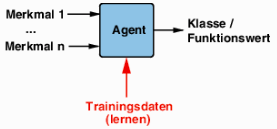
\includegraphics[scale=1]{lernenderagent.png}
                   \captionof{figure}{lernender Agent}
                   \raggedleft\footnotesize\cite[S.194, Abb. 8.4(rechts)]{ertel2016}
                   %\quelle W. Ertel, Grundkurs künstliche Intelligenz, Springer Fachmedien, 2016, S. 194, Abb. 8.4 (rechts)
                \end{Figure}
                Die \emph{Aufgabe} des \emph{lernenden Agenten} ist das lernen einer Abbildung von einem Merkmalsvektor auf eine Klasse oder einen stetigen Funktionswert anhand von \emph{Trainingsdaten}. Es muss im Vorfeld festgelegt werden, welche Art von Agent, das heißt welches Lernverfahren, eingesetzt wird (siehe Abschnitt \ref{sec:perzeptron}, S. \pageref{sec:perzeptron} \emph{Perzeptron} und Abschnitt \ref{subsec:nn-methode}, S. \pageref{subsec:nn-methode} \emph{Nearest Neighbour Methoden}).
                Bei der Auswahl der Trainingsdaten ist zu beachten, dass diese repräsentativ für die zu lernende Aufgabe sind, da die gelernte Abbildung ansonsten nur schlecht auf unbekannte Daten generalisiert.\\
                Nachdem der Agent eine Abbildung anhand von Trainingsdaten gelern hat, muss diese anhand eines geeigneten \emph{Leistungsmaßes} unter Verwendung von \emph{Testdaten} evaluiert werden. \emph{Testdaten} sind dabei Merkmalsvektoren, für die  die richtige Klasseneinteilung oder der richtige Funktionswert bereits bekannt sind, die aber keine Trainingsdaten waren.\cite{ertel2016}

            \subsection{Eager Learning}
                Als \emph{Eager Learning} werden solche Lernverfahren bezeichnet, bei denen in einem ersten Schritt in einer (in der Regel aufwändigen) Lernphase bestehendes Wissen aus den Trainingsdaten in Form einer Abbildung extrahiert wird.
                Der in der Lernphase betriebene Aufwand rechnet sich aber in der Anwendung, da diese Klasse von Lernverfahren, sobald die Abbildung gelernt wurde, sehr effizient auf neue, ungesehene Daten angewendet werden kann.\cite{ertel2016} 

        \section{Das Perzeptron}
        \label{sec:perzeptron}
            In diesem Abschnitt der Arbeit soll mit dem \emph{Perzeptron} ein einfaches, aber dennoch aufschlussreiches Beispiel für eine konkrete Implementierung eines lernenden Agenten gegeben werden.
            \newline
            Das Perzeptron ist ein \emph{linearer Klassifizierer}, das heißt, es ist in der Lage, einen Eingabevektor auf eine von zwei Klassen abzubilden, sofern es eine Hyperebene gibt, die die beiden Klassen voneinander trennt.\cite{ertel2016}

            \subsection{Linear separable Mengen}
            \label{subsec:lernverfahren}
                Zunächst soll verdeutlicht werden, was es heißt, dass zwei Mengen durch eine Hyperebene voneinander getrennt werden.
                Hierzu führen wir den Begriff der 
                \emph{linear separablen Mengen} ein.
                \newline
                Zwei Mengen $M_1 \subset \mathbb{R}^n$ und $M_2 \subset \mathbb{R}^n$ heißen \emph{linear separabel} genau dann, wenn es eine Schwelle $\theta$ und reelle Zahlen $a_1,\dots,a_n$ gibt, sodass
                $$
                    \sum_{i=1}^n a_ix_i > \theta \forall x \in M_1$$
                und
                $$\sum_{i=1}^n a_ix_i \leq \theta \forall x \in M_2$$
                gilt.\cite{ertel2016}
                \newline
                In der Terminologie der linearen Algebra beduetet dies, es existiert eine $n-1$ dimensionale Hyperebene, die durch die Gleichung
                $$
                    \sum_{i=1}^n a_ix_i = \theta
                $$
                definiert wird und die die beiden Mengen $M_1$ und $M_2$ voneinander trennt.

            \subsection{Abbildungsvorschrift}
                Wie bereits erwähnt handelt es sich beim \emph{Perzeptron} um einen linearen Klassifizierer, der genau die linear separablen Mengen klassifizieren kann. Das heißt, das Perzeptron ist eine Abbildung eines Eingabevektors $x$ auf einen diskreten Klassenwert. Es wird definiert durch die Abbildungsvorschrift
                $$
                    P(x)=\left\{\begin{array}{cl} 1, & \mbox{falls }\sum_{i=1}^nw_ix_i > 0\\ 0, & \mbox{falls} \sum_{i=1}^n w_ix_i \leq 0 \end{array}\right. \text{ \footnotesize\cite[S.201]{ertel2016}} 
                $$

                Aus der Abbildungsvorschrift wird ersichtlich, dass $n$ Skalare, $w_1,\dots,w_n$ benötigt werden. Der Vektor $w = (w_1,\dots, w_n)$ wird als \emph{Gewichtsvektor} bezeichnet. Dieser Gewichtsvektor $w$ ist im Allgemeinen zunächst unbekannt und muss in einem vorgelagerten Schritt gelernt werden.

            \subsection{Lernverfahren}
                Eine Möglichkeit, den Gewichtsvektor $w$ zu ermitteln, stellt der Algorithmus PerzeptronLernen dar, der in diesem Abschnitt vorgestellt werden soll. Der Algorithmus PerzeptronLernen nimmt als Eingabe zwei Mengen $M_+$ und $M_-$, wobei die Menge $M_+$ Eingabevektoren enthält, von denen bereits bekannt ist, dass sie mit $1$ klassifiziert werden sollen. Analog enthält die Menge $M_-$ Eingabevektoren, von denen bereits bekannt ist, dass sie mit $0$ klassifiziert werden sollen.
                \newline
                Nun wird ein beliebiger initialer Gewichtsvektor $w$ gewählt.
                \newline
                Für alle Elemente $x \in M_+$ wird geprüft, ob $w \cdot x := \sum_{i=1}^nw_ix_i \leq 0$ erfüllt ist. Ist dies der Fall, so folgt, dass das Element $x$ falsch klassifiziert wurde, der Gewichtsvektor $w$ also noch nicht richtig sein kann. Folglich wird der Gewichtsvektor $w$ angepasst, indem der Wert des falsch klassifizierten Elementes $x \in M_+$ komponentenweise aufaddiert wird.
                \newline
                Analog wird für die Elemente aus $M_-$ vorgegangen, nur das hier geprüft wird, ob $\sum_{i=1}^nw_ix_i > 0$ gilt und $w$ gegebenfalls durch Substraktion des Wertes des Eingabevektros $x$ angepasst wird.

                \subsubsection{Algorithmus PerzeptronLernen}
                    \begin{algorithm}[H]
                        \KwData{$M_+,M_-, w \in\mathbb{R}^n$ beliebig}
                        \KwResult{Gewichtsvektor $w$}
                        \Repeat{Alle Vektoren $\in M_+ \cup M_-$ korrekt klassifiziert}{
                            \For{$x \in M_+$}{
                                \If{$w\cdot x \leq 0$}{$w = w + x$}
                            }
                            \For{$x \in M_-$}{
                                \If{$w\cdot x > 0$}{
                                    $w = w -x$
                                }
                            }
                        }
                        \caption{PerzeptronLernen nach \cite[S.202]{ertel2016}}
                    \end{algorithm}
                
                    \subsubsection{Beispiel}
                        Das Vorgehen des Lernverfahrens soll im Folgenden anhand eines einfachen Beispiels verdeutlicht werden.\footnote{siehe \cite{ertel2016}, S. 202, Beispiel 8.2}\footnote{Abbildungen \ref{fig:bspPL1}, \ref{fig:bspPL2}, \ref{fig:bspPL3}, \ref{fig:bspPL4}, \ref{fig:bspPL5} angelehnt an \cite[S.203, Abb. 8.10]{ertel2016}}
                        \newline
                        Als Trainingsdaten dienen die Mengen $M_+ = \{(0,1.8),(2,0.6)\}$ und \newline $M_- = \{(-1.2,1.4),(0.4,-1)\}$, als initialer Gewichtsvektor $w$ dient $(1,1)$.\\
                        1. Durchlauf:\\
                        $M_+$\\
                        $(1,1)\cdot(0,1.8) = 1.8 > 0 \rightarrow $ erster Vektor korrekt klassifiziert.\\
                        $(1,1)\cdot(2,0.6) = 2.6 > 0 \rightarrow$ zweiter Vektor korrekt klassifiziert\\
                        $M_-$\\
                        $(1,1)\cdot(-1.2,1.4) = 0.2 > 0 \rightarrow$ dritter Vektor falsch klassifiziert\\
                        $\rightarrow w_{neu} = (1,1)-(-1.2,1.4) = (2.2,-0.4)$\\
                        $(2.2,-0.4) \cdot (0.4,-1) = 1.28 > 0 \rightarrow$ vierter Vektor falsch klassifiziert\\
                        $\rightarrow w_{neu} = (2.2,-0.4)-(0.4,-1) = (1.8,0.6)$

                        \begin{Figure}
                            \begin{minipage}[b]{.4\linewidth}
                                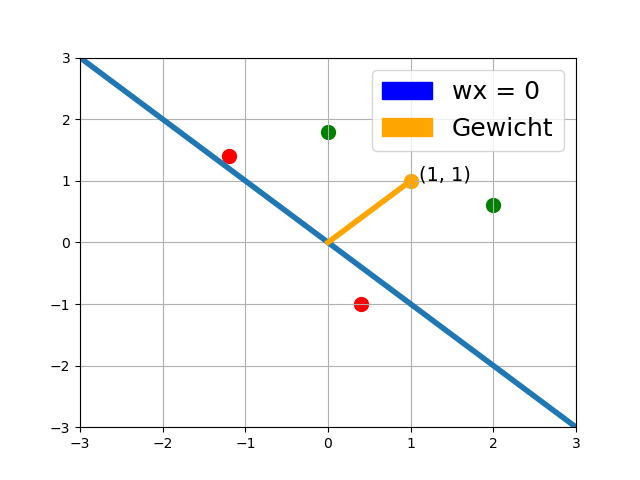
\includegraphics[scale=0.5]{bsp1.png}
                                \captionof{figure}
                                {Situation vor Iteration 1, x-Achse: 1. Komponente, y-Achse: 2. Komponente}
                                \label{fig:bspPL1}   
                            \end{minipage}
                            \hspace{.1\linewidth}
                            \begin{minipage}[b]{.4\linewidth}
                                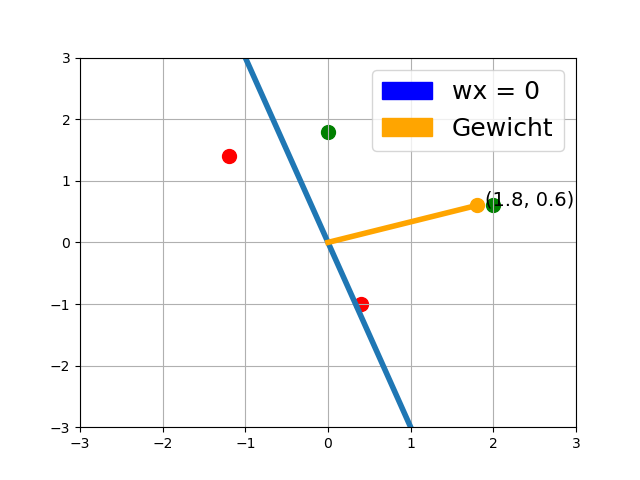
\includegraphics[scale=0.5]{bsp2.png}
                                \captionof{figure}{Situation nach Iteration 1 \newline\newline}
                                \label{fig:bspPL2}    
                            \end{minipage}
                        \end{Figure}

                        2. Durchlauf:\\
                        $M_+$\\
                        $(1.8,0.6)\cdot (0,1.8) = 1.08 > 0 \rightarrow$ erster Vektor korrekt klassifiziert.\\
                        $(1.8,0.6)\cdot (2,0.6) = 3.96 > 0 \rightarrow$ zweiter Vektor korrekt klassifiziert.\\
                        $M_-$\\
                        $(1.8,0.6)\cdot (-1.2,1.4) = -1.32 \leq 0 \rightarrow$ dritter Vektor korrekt klassifiziert.\\
                        $(1.8,0.6)\cdot (0.4,-1) = 0.12 > 0 \rightarrow$ vierter Vektor falsch klassifiziert.\\
                        $\rightarrow w_{neu} = (1.8,0.6)-(0.4,-1) = (1.4,1.6)$\\
                        \\
                        3. Durchlauf:\\
                        $M_+$\\
                        $(1.4,1.6)\cdot (0,1.8) = 2.88 > 0 \rightarrow$ erster Vektor korrekt klassifiziert.\\
                        $(1.4,1.6)\cdot (2,0.6) = 3,76 > 0 \rightarrow$ zweiter Vektor korrekt klassifiziert.\\
                        $M_-$\\
                        $(1.4,1.6) \cdot (-1.2,1.4) = 0,56 > 0 \rightarrow$ dritter Vektor falsch klassifiziert.\\
                        $\rightarrow w_{neu} = (1.4,1.6)-(-1.2,1.4) = (2.6,0.2)$\\
                        $(2.6,0.2)\cdot (0.4,-1) = 0.84 > 0 \rightarrow$ vierter Vektor falsch klassifiziert.\\
                        $\rightarrow w_{neu} = (2.6,0.2)-(0.4,-1) = (2.2,1.2)$\\
                        \begin{Figure}
                            \begin{minipage}[b]{.4\linewidth}
                                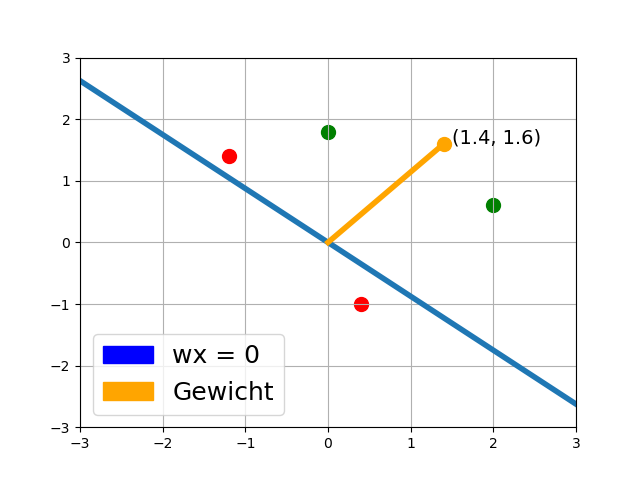
\includegraphics[scale=0.5]{bsp3.png}
                                \captionof{figure}{Situation vor Iteration 3} 
                                \label{fig:bspPL3}
                            \end{minipage}
                            \hspace{.1\linewidth}
                            \begin{minipage}[b]{.4\linewidth}
                                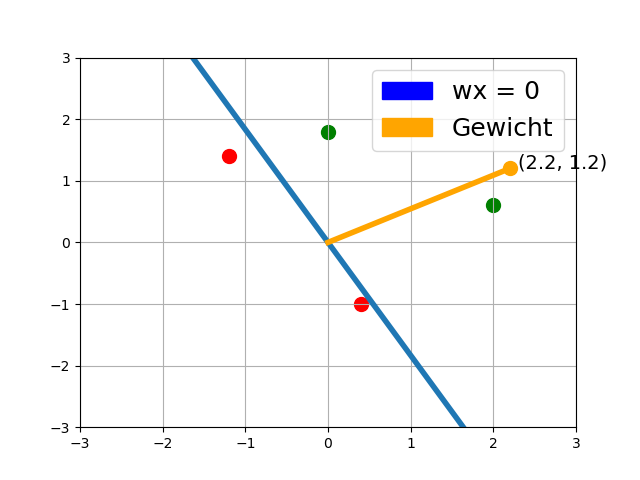
\includegraphics[scale=0.5]{bsp4.png}
                                \captionof{figure}{Situation nach Iteration 3}
                                \label{fig:bspPL4}    
                            \end{minipage}     
                        \end{Figure}
                        4. Durchlauf:\\
                        $M_+$\\
                        $(2.2,1.2)\cdot (0,1.8) = 2.16 > 0 \rightarrow$ erster Vektor korrekt klassifiziert.\\
                        $(2.2,1.2)\cdot (2,0.6) = 5.12 > 0 \rightarrow$ zweiter Vektor korrekt klassifiziert.\\
                        $M_-$\\
                        $(2.2,1.2)\cdot (-1.2,1.4) = -0.96 \leq 0 \rightarrow$ dritter Vektor korrekt klassifiziert.\\
                        $(2.2,1.2)\cdot (0.4,-1) = -0,32 \leq 0 \rightarrow$ vierter Vektor korrekt klassifiziert.
                        \begin{Figure}
                            \centering
                            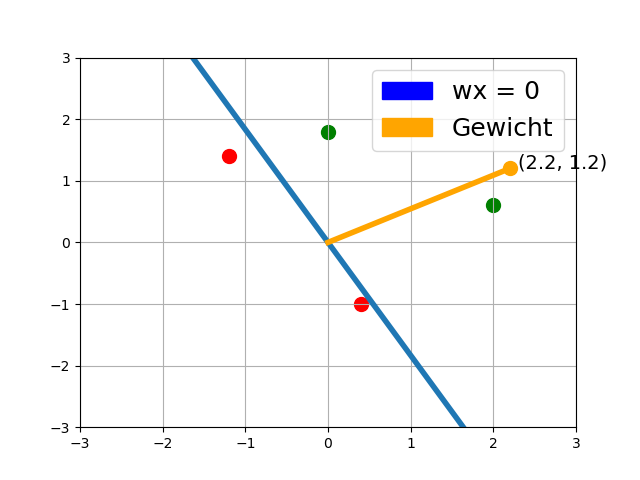
\includegraphics[scale=0.5]{bsp4.png}
                            \captionof{figure}{Situation nach Terminierung des Lernverfahrens}
                            \label{fig:bspPL5}    
                        \end{Figure}
                        Der Gewichtsvektor $w = (2.2,1.2)$, klassifiziert alle Elemente der Trainingsdaten korrekt, der Lernalgorithmus terminiert und gibt $w = (2.2,1.2)$ als Ergebnis zurück.\\
                        Die Abbildungen \ref{fig:bspPL1}, \ref{fig:bspPL2}, \ref{fig:bspPL3}, \ref{fig:bspPL4} und \ref{fig:bspPL5} veranschaulichen, wie eine Anpassung des Gewichtsvektors $w$ die Trennebene beeinflusst.
                        Zu beachten ist auch, dass der richtige Vektor bereits in der vorletzten Iteration gefunden wird. Da dieser Vektor aber noch auf allen Trainingsdaten getestet werden muss bedarf es einer weiteren Iteration.

                    \subsubsection{Finden guter Initialwerte für $w$}
                    Die asymptotische Laufzeitanalyse des Algorithmus PerzeptonLernen in Abhängigkeit der Eingabegröße $n$, wobei $n$ der Anzahl der Trainingsdaten entspricht, gestaltet sich als schwierig. Einzig das Best-Case-Szenario, bei dem der initiale Gewichtsvektor so gewählt wird, dass es keiner Anpassung bedarf, lässt sich asymptotisch mit $\Omega(n)$ nach unten abschätzen, da jedes Element aus den Trainingsdaten, also $M_+ \cup M_-$, mindestens einmal überprüft werden muss. Für die Average-Case und Worst-Case Laufzeiten lässt sich so jedoch keine Aussage treffen, da die Wahl von $w$ deutlich größere Auswirkungen auf die Laufzeit des Lernverfahrens hat.
                    Folglich kann die Laufzeit des Algorithmus bei Verwendung eines optimalen intialen Gewichtsvektors $w$ auf $\mathcal{O}(n)$ reduziert werden. Allerdings entspricht das Finden optimaler Gewichtsvektoren genau dem Ausführen des Lernverfahrens, dieses hat schließlich zum Ziel, ein $w$ zu finden, das die Mengen trennt, was äquivalent dazu ist, dass das $w$ bei Verwendung als initialem Gewichtsvektor im Lernverfahren nicht mehr angepasst werden muss, da es alle Trainingsdaten korrekt klassifiziert.
                    Ein finden optimaler Gewichtsvektoren ist also keine Option zu Verbesserung der Laufzeit.
                    \newline
                    Dennoch lassen sich durch die Verwendung heuristisch bestimmter \glqq guter\grqq\  Gewichtsvektoren $w$ im Durchschnitt Laufzeitverbesserungen erreichen.
                    Eine geeignete Heuristik sieht wie folgt aus: 
                    \newline
                    Alle $x\in M_+$ werden aufaddiert und davon wird die Summer aller $x\in M_-$ abgezogen.
                    $$
                        w = \sum_{x \in M_+}x - \sum_{x \in M_-}x \text{ \footnotesize\cite[S.206]{ertel2016}}
                    $$

            \subsection{Erweiterung auf linear affine Mengen}
                Die bisherige Abbildungsvorschrift des Perzeptrons beruht darauf, dass die beiden Mengen durch eine Hyperebene durch den Nullpunkt trennbar sind. Dies widerspricht aber der Definition linear separabler Mengen, die lediglich voraussetzt, dass es eine beliebige Schwelle, insbesondere also auch solche ungleich $0$ (vgl. Abschnitt \ref{subsec:lernverfahren} ) existiert. Daher stell sich unweigerlich die Frage, ob das Perzeptron tatsächlich alle linear separablen Mengen korrekt klassifizieren kann, oder lediglich solche, die durch eine durch den Ursprung verlaufende Hyperebene trennbar sind. Um zu zeigen, dass das Perzeptron auch solche Mengen, die durch eine durch eine beliebige Schwelle definierte Hyperbene trennbar sind, korrekt klassifizieren kann, greifen wir auf die bekannten Rechenregeln der reellen Zahlen für Ungleichungen zurück.
                Zunächst erweitern wir den Eingabevektor $x$ um eine $n+1$. Komponente, die Konstant auf $-1$ gesetzt wird.\cite{ertel2016}
                \newline 
                Damit ergibt sich für die Abbildungsvorschrift des Perzeptrons 
                $$
                    P(x)=\left\{\begin{array}{cl} 1, & \mbox{falls }\sum_{i=1}^nw_ix_i - w_{i+1} > 0\\ 0, & \mbox{falls} \sum_{i=1}^n w_ix_i - w_{i+1} \leq 0 \end{array}\right. 
                $$
                und für die Gleichung der trennenden Hyperebene
                $$
                    \sum_{i=1}^nw_ix_i - w_{i+1} = 0
                $$
                Durch einfache Äquivalenzumformung ergibt sich die folgende Gleichung für die Hyperebene
                    $$
                        \sum_{i=1}^nw_ix_i = w_{i+1}
                    $$
                    Daraus folgt für die Abbildungsvorschrift des Perzeptrons:
                    $$
                    P(x)=\left\{\begin{array}{cl} 1, & \mbox{falls }\sum_{i=1}^nw_ix_i > w_{i+1}\\ 0, & \mbox{falls} \sum_{i=1}^n w_ix_i \leq w_{i+1} \end{array}\right. 
                    $$
                    Mit $w_{i+1}$ ist also eine neue Schwelle ungleich $0$ gefunden, die das Gewünschte liefert. Damit ist gezeigt, dass das Perzeptron auch solche Mengen klassifizieren kann, die durch eine nicht durch den Nullpunkt verlaufende Hyperebene voneinander getrennt werden können. Damit ist das Perzeptron in der Lage tatsächlich alle linear separablen Mengen zu klassifizieren.
                    \newline
                    Zu beachten ist, dass der Schwellwert $w_{i+1}$ zunächt unbekannt ist, und erst im Verlaufe des Lernverfahrens zusammen mit dem Gewichstsvektor $w$ gelernt wird.\cite{ertel2016}
                
            \subsection{Probleme des Perzeptrons}
                        Zwar ist das Perzeptron äquivalent zu \emph{zweilagigen neuronalen Netzen}\cite{ertel2016}, doch die Einschränkung auf \emph{linear separable Mengen} bringt das Perzeptron bereits bei relativ einfachen Beispielen an seine Grenzen.
            % Obwohl das Perzeptron ein sehr einfaches maschinelles Lernverfahren ist, so hat es in der Praxis, außer als Vorstufe zu neuronalen Netzen, keine Bedeutung. Aufgrund der Einschränkung auf linear seprablen Mengen stößt das Perzeptron schnell an seine Grenzen.
                    Zur Verdeutlichung soll das folgende Beispiel betrachtet werden:
                    \newline
                    Gehen wir davon aus, dass das Perzeptron die booleschen Funktionen lernen soll. Das heißt es sollen Abbildungen der Form $$\{0,1\}\times\{0,1\} \rightarrow \{0,1\}$$ gelernt werden.
                    Zunächst betrachten wir die logische UND-Funktion, das heißt die Abbildung
                    $$
                        f:\{0,1\}\times\{0,1\}\rightarrow\{0,1\}: x\mapsto f(x)
                    $$
                    mit
                    $$
                        f(x)=\left\{\begin{array}{cl} 1, & \mbox{falls }x=(1,1)\\
                        0, & \mbox{sonst}\end{array}\right. 
                    $$
                    % Bild
                    \begin{Figure}
                        \begin{minipage}[b]{.4\linewidth}
                            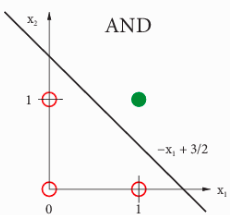
\includegraphics[scale=0.5]{AND.png}
                            \captionof{figure}{Hyperebene, die die mit $1$ und $0$ klassifizierten Elemente voneinander trennt}
                            \raggedleft\footnotesize\cite[S.201, Abb. 8.8(links)]{ertel2016}                      \label{fig:and}
                                % \quelle W. Ertel, Grundkurs künstliche Intelligenz, Springer Fachmedien, 2016, S. 201, Abb. 8.8(links)    
                        \end{minipage}
                        \hspace{.1\linewidth}
                        \begin{minipage}[b]{.4\linewidth}
                            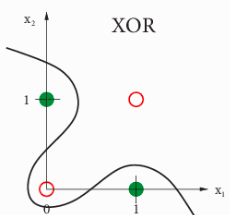
\includegraphics[scale=0.5]{XOR.png}
                            \captionof{figure}{Versuch, die Klassen zu trennen\newline\newline}
                            \raggedleft\footnotesize\cite[S.201, Abb. 8.8(rechts)]{ertel2016}
                            \label{fig:xor}
                            % \quelle W. Ertel, Grundkurs künstliche Intelligenz, Springer Fachmedien Wiesbaden, 2016, S. 201, Abb. 8.8 (rechts)
                        \end{minipage}
                    \end{Figure}
                    An Abb. \ref{fig:and} wird deutlich, dass die Menge der Vektoren, die auf $1$ abbilden durch eine linear affine Hyperebene von der Menge der Vektoren, die auf $0$ abbilden, getrennt wird.
                    \newline
                    Anders verhält es sich bei der logischen XOR-Funktion:
                    $$
                        f:\{0,1\}\times\{0,1\}\rightarrow\{0,1\}: x\mapsto f(x)
                    $$
                    mit
                    $$
                        f(x)=\left\{\begin{array}{cl} 1, & \mbox{falls }x=(1,0) \vee x = (0,1)\\
                        0, & \mbox{sonst}\end{array}\right. 
                    $$
                    % Bild
                    Auch in diesem Fall wird durch einen Blick auf den Graphen (Abb. \ref{fig:xor}) deutlich, dass es keine Möglichkeit gibt, die Menge der Vektoren, die auf $1$ abbilden durch eine Hyperebene, die der Gleichung der Form
                    $$
                        \sum_{i=1}^nw_ix_i = \theta
                    $$
                    genügt, von der Menge der Vektoren, die auf $0$ abbilden, zu trennen.\cite{ertel2016}
                    \newline
                    Anhand dieses Beispiels wird deutlich, dass das Perzeptron bei weitem nicht so mächtig ist wie andere maschinelle Lernverfahren (vgl Abschnitt \ref{sec:nnl}, S. \pageref{sec:nnl} und \cite{ertel2016} Kapitel 9 \glqq Neuronale Netze \grqq ).

% Ende mein Teil
                        
        \section{Grundbegriffe und Abstandsfunktionen}
            \subsection{Was ist Ähnlichkeit?}
                Als Ähnlichkeit wird häufig bezeichnet, wenn in zwei oder mehr beobachteten Objekten, in zu untersuchenden Ausprägungen, Übereinstimmungen zu finden sind.\par
                Hierzu passend ist das Beispiel eines Arztes, der sich während einer Diagnose eines seiner Patienten daran erinnert, bereits in der Vergangenheit bei anderen Patienten die gleichen Symptome beobachtet zu haben.\cite{ertel2016} Durch das Erinnern an einen Fall in der Vergangenheit und den enstandenden Vergleich zur Gegenwart, ist es dem Arzt möglich seinem momentanen Patienten zu helfen, da die gleichen Behandlungsmethoden verwenden werden können.\par
                Weil für Menschen Ähnlichkeit intuitiver ist als für Maschinen stellt sich die Frage, wie man einer Maschine vermitteln kann, wann Objekte zueinander ähnlich sind und vor allem, wie man dieses Konzept in eine für Maschinen verständliche Sprache übersetzt und umgesetzt werden kann.\par
                Zu diesem Zwecke wird die aus der Mathematik bekannte Datenstruktur der Vektoren betrachtet.
                %Um diese Frage beantworten zu können, betrachten mit einer aus der Mathematik bekannten Datenstruktur der Vektoren.

                Vektoren sind in diesem System Tupel von Daten. Innerhalb dieses Systems werden Vektoren mit Werten der reellen Zahlen verwendet und für Werte aus anderen Räumen wird eine eindeutige Repräsentation gesucht.\par Beispielsweise könnte eine Übersetzung von Zeichenketten in den reellen Raum über ein ASCII-System erfolgen.\par 
                Für unsere Anwendung wird die Eigenschaft ausgenutzt, dass Vektoren Elemente des Raumes $\mathbb{R}^n$ sind, wobei jede der $n$ Dimensionen für eine konkrete Ausprägung einer Eigenschaft steht. Damit lassen sich Datenmengen als Punkte in einem $\mathbb{R}^n$ dimensionalen Hyperraum darstellen. Dadurch definiert Wolfgang Ertel: \glqq Zwei Beispiele sind umso ähnlicher, je geringer ihr Abstand im Merkmalsraum ist.\grqq \cite[S. 207]{ertel2016} %[1.1]
            \subsection{Einführung von Abstandsfunktionen}
                Innerhalb des definierten, metrischen $n$-dimensionalen Merkmalsraumes kann man infolgedessen die Unterschiedlichkeit zweier betrachteter Objekte mithilfe einer Abstandsfunktion bestimmen. Somit kennen wir die Ähnlichkeit zweier Datenpunkte zueinander, wenn der Abstand zwischen ihnen im Merkmalsraum bekannt ist.\par Hierzu bieten sich eine Vielzahl an Metriken an, z.B. die euklidische Norm, Manhattan-Abstand, als auch der Hamming-Abstand. Weitere erwähnenswerte Metriken lauten: Summe der Abstandsquadrate, Abstand der maximalen Komponente.\par 
                Als \emph{metrischen Raum} bezeichnet man eine Menge in der eine Abstandsfunktion $D(x,y)$ mit $x,y \in \mathbb{R}^n$ definiert ist.\par
                Folglich kann man, innerhalb dieser definierten Menge, zwischen Elementen Abstände bestimmen, was sich besonders nützlich für die im Folgenden behandelten Anwendungen erweist. \par
                Ein Entwickler muss sich zusätzlich bei der Auswahl einer Metrik im Klaren sein, welche Abstandsfunktion für seine Anwendung am besten geeignet ist.
            \subsection{Euklidische Norm}
                Eine namenhafte Abstandsfunktion, die meist mit dem Satz des Pythagoras eingeführt und berechnet werden kann, ist die der euklidischen Norm und ist wie folgt definiert:
                $$
                    x,y \in \mathbb{R}^n
                $$
                $$
                    d_e(x,y):= |x - y| = \sqrt{\sum_{i=1}^{n}(x_i -y_i)^2} \text{ \footnotesize\cite[S.207]{ertel2016}}
                $$

                In unterschiedlichen Anwendungsfällen können bestimmte Merkmale eine wichtigere Rolle spielen als andere.\cite{ertel2016} Dazu wird die euklidische Norm um einen Gewichtsvektor $w$ erweitert, wobei dieser die Gewichtung jeder einzelnen Komponente bestimmt.\par Eine gewichtete Variante der euklidischen Norm sieht wie folgt aus:\par
                $$
                    w,x,y \in \mathbb{R}^n
                $$
                $$
                    d_w(x,y):= |x - y| = \sqrt{\sum_{i=1}^{n}w_i(x_i -y_i)^2} \text{ \footnotesize\cite[S.207]{ertel2016}}
                $$     

            
            \subsection{Manhattan-Abstand}
                Hierbei werden nur Geraden, die parallel zu einer Ursprungsachse verlaufen betrachtet, um zwei Punkte zu verbinden. Die Distanz ergibt sich aus der aufsummierten Gesamtlänge jeder der dabei verwendeten Geraden.\par 
                %Hierbei bewegt man sich nur auf der horizontalen und vertikalen Ebene, um zwei Punkte zu verbinden. 
                Formal beschreibt der \emph{Manhattan-Abstand}, dass die Distanz zwischen zwei Elementen aus einem mehrdimensionalen Raum den Differenzen jeder Komponente als absoluten Wert aufsummiert entspricht.\par %, der verwendeten Geraden.\par

				
                In Formelnotation sieht der \emph{Manhattan-Abstand} wie folgt aus:
                $$
                    x,y \in \mathbb{R}^n 
                $$
                $$
                    d_m(x,y):= \sum_{i=1}^{n} |x_i -y_i| \text{ \footnotesize\cite[S.245]{ertel2016}}
                $$

                Ein Beispiel hierfür ist in Abbildung \ref{fig:manhattan} zu sehen, wobei die folgenden Daten gegeben sind:\par
                   $x,y \in \mathbb{R}^2$ mit $x= (2, 2)$ und $y= (5,4)$
                \begin{Figure}
                    \centering
                    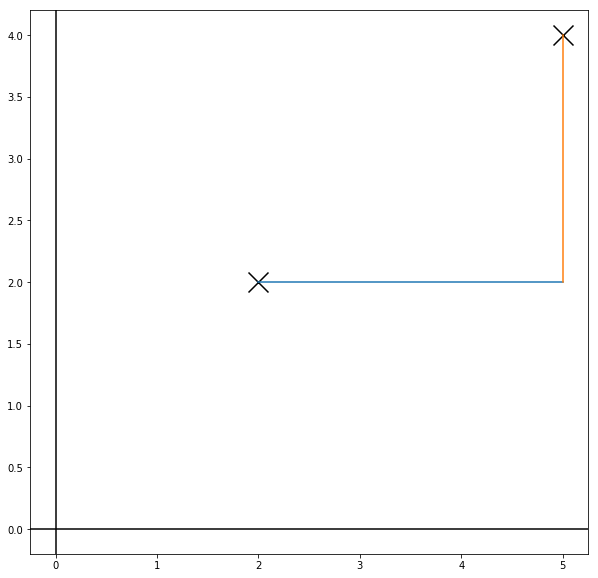
\includegraphics[scale=0.3]{manhattanDistance.png}
                   \captionof{figure}{Beispiel Manhattan-Abstand}
                   \label{fig:manhattan}
                \end{Figure}    
              	Für die Distanz ergibt sich dadurch: $d_m(x,y)= |2-5|+|2-4|=|-3|+|-2|=5$                  
                                %**Noch eine Erklärung zum Schaubild**\par        

                         
            \subsection{Hamming-Abstand}
                Ist ein Abstandsmaß, dass bei Zeichenketten häufig Verwendung findet und gibt die Unterschiedlichkeit zwischen zwei endlichen Elementen aus einem Zeichenraum $\Sigma$ als Wert wieder.
                $$ x,y \in \Sigma^n $$
                $$ d_h(x,y):= |\{x_i \neq y_i \}|, i \in \{1,\dots,n\}$$
                Es folgt ein Beispiel, wie der \emph{Hamming-Abstand} zwischen zwei Zeichenketten (hier: Binärzahlen) aussehen würde.\par
                $\sum=\{0,1\}$ als Alphabet.\par
                $x = 01101$\par
                $y= 10001$\par
                $D_h(x,y)=3$, da wir nur an den Stellen $i=\{1,2,3\}$ also in $ x_1,x_2,x_3$ Unterschiede zu $y_1,y_2,y_3$ vorfinden.
                        
            \subsection{Lazy Learning Lernverfahren}  
                Stehen im Gegensatz zu den \emph{Eager Learning Lernverfahren}. Das \emph{Lazy Learning} heißt übersetzt faules Lernen und ist eine weitere Kategorie von Lernverfahren. Diese Art von Verfahren sind gekennzeichnet dadurch, dass es genügt, alle vorhandenen Trainingsdaten in eine vom System verwendete Datenstruktur zu sichern. Es wird keine Klassifikationsabbildung ermittelt, wie bei dem \emph{Eager Learning}. % dass der Großteil der benötigten Rechenzeit nicht wie beim eager Learning zum Ermitteln einer Klassifikationsabbildung verwendet wird, sondern es genügt alle Trainingsdaten in eine vom System verwendete Datenstruktur zu sichern. 
                            
            % \subsection{Trainingsdaten}
                % Sind Daten, deren    korrekte Klassifikation   bekannt ist und werden meist von Experten vorgegeben.
                % Ein Beispiel hierfür wäre, die zur Klassifikation benötigten Trainingsdaten einer Apfelsortiermaschine, bestehend aus Größe und Farbe.[1.3]
                % Nachdem uns ein Experte vorgibt, wie eine Apfelsorte auszusehen hat versucht unser System, abhängig vom Typ des Algorithmus, selbstständig eine Generalisierung vorzunehmen. 
                        
        \section{Nearest-Neighbour Lernverfahren}
        \label{sec:nnl}
            Gehört zu den faulen Lernverfahren, da initial außer dem Abspeichern der Trainingsdaten kein zusätzlicher Rechenaufwand betrieben wird. Als Ziel des Systems kann man bezeichnen, dass mittels Trainingsdaten versucht wird, neue Daten zu klassifizieren bzw. einordnen zu können. (Vgl. Kapitel \ref{subsec:lernenderagent}, lernender Agent auf S. \pageref{subsec:lernenderagent})
                        
            \subsection{Nearest-Neighbour Methode}
            \label{subsec:nn-methode}
                Einführend werden zur Anschaulichkeit nur zwei mögliche Klassen, denen ein Datenpunkt zugeordnet werden kann, betrachtet. Jedoch kann die Methode des \emph{nearest Neighbour} problemlos auf mehr Klassen erweitert werden.\par
                Unsere Datenpunkte sind Vektoren des $\mathbb{R}^n$, wobei jede Komponente einer konkreten Ausprägung entspricht.\par
                Beispielsweise könnte der Versuch einen Patienten mittels eines Vektors darzustellen wie folgt aussehen. Indem man jeder Komponente des Vektors eine konkrete Ausprägung des Patienten zuordnet, wie z.B. einer Komponente das Alter oder die Größe der Person, kann auf diese Weise ein Vektor einen Patienten repräsentieren und alle für unser System benötigten Informationen enthalten.\par
                Zu Beginn werden die Mengen $M_+$ und $M_-$ als Trainingsdaten, $s$ als den zu klassifizierenden Datenpunkt und $t$ als den nächsten Nachbarn von $s$ definiert. Die Funktion \emph{argmin\{\}} erhält eine endliche Menge als Eingabe und gibt die Stelle an dem ein Minimum auftritt als Rückgabewert zurück. Analog würde für \emph{argmax\{\}} gelten, dass die Stelle an der ein Maximum auftritt zurückgegeben wird.\par
                        
                Die Idee des \emph{nearest Neighbour} Verfahrens ist, wenn der nächste Nachbarn von $s$ erfolgreich bestimmt werden konnte, kann aufgrund der Ähnlichkeit zwischen beiden Datenpunkten die Aussage getroffen werden, dass $s$ vermutlich der gleichen Klasse angehört wie $t$. Dadurch ist unsere Klassifizierung erfolgt.
                \newpage
               
                        
            \subsection{Nearest-Neighbour Algorithmus}
            \label{subsec:nnalgo}
             Der Algorithmus ist wie folgt definiert:\par
                            \begin{algorithm}[H]
                                \KwData{$M_+,M_-,s \in \mathbb{R}^n$}
                                \KwResult{Klassifikation von $s$}
                                    \For{$x \in M_+ \cup M_-$}{
                                        $d(s,x)$\;
                                    }
                                    	$t= argmin$\{$d(s,x)$\}\;
                                    \eIf{$t \in M_+$}{
                                        \KwRet{+}\;
                                    }
                                    {
                                        \KwRet{-}\;
                                    }
                                \caption{Nearest Neighbour Algorithm nach \cite[S.208]{ertel2016}}
                            \end{algorithm}
				
				Als Nächstes wird das \emph{nearest Neighbour} Verfahren anhand eines Beispiels ausgeführt.
				In Abb. \ref{fig:nn1} sind zwei Klassen \{rot, grün\} sind als Trainingsdaten vorgegeben und dazu ein schwarzer Punkt dessen Klasse ermittelt werden soll. Alle Daten sind Teil des Raumes $\mathbb{R}^2$.\par
                %Bilder Nearst Neighbour
                \begin{Figure}
                    \begin{minipage}[b]{.4\linewidth}
                        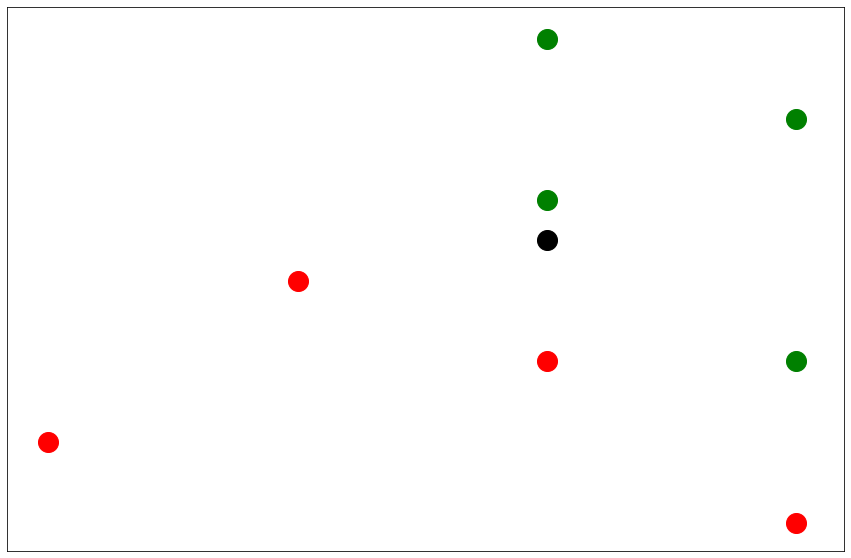
\includegraphics[width=\linewidth]{nn1.png}
                        \captionof{figure}{Ausgangssituation}\label{fig:nn1}       
                    \end{minipage}
                    \hspace*{.1\linewidth}
                    \begin{minipage}[b]{.4\linewidth}
                        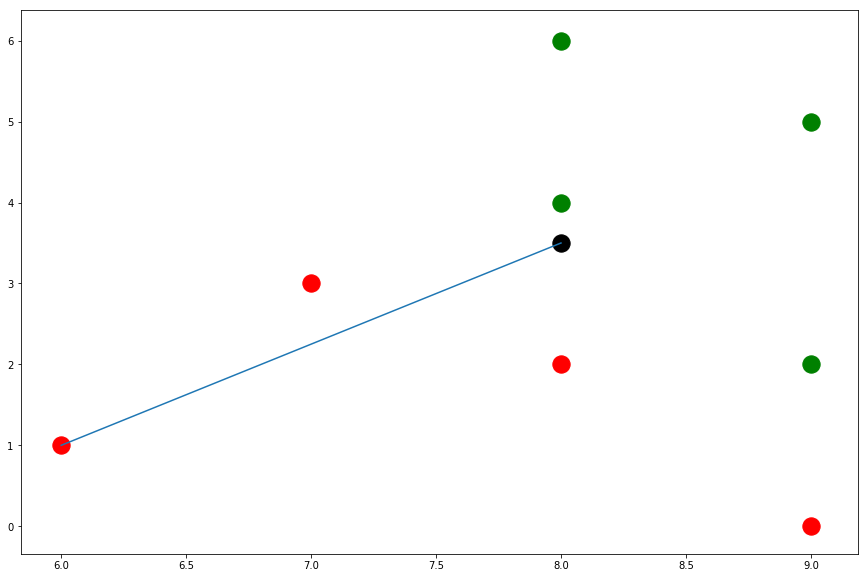
\includegraphics[width=\linewidth]{nn2.png}
                        \captionof{figure}{Bestimmen des ersten Abstands}   \label{fig:nn2} 
                    \end{minipage}
                \end{Figure}

                Im nächsten Schritt wird die Distanz mithilfe der gewählten Abstandsfunktion (hier: euklidische Norm) zwischen Ausgangspunkt und jedem Punkt innerhalb des Merkmalsraumes bestimmt. In den Abbildungen \ref{fig:nn2}, \ref{fig:nn3} und \ref{fig:nn5} als blau gekennzeichnet. 
                        
                
                \begin{Figure}
                    \begin{minipage}[b]{.4\linewidth}
                        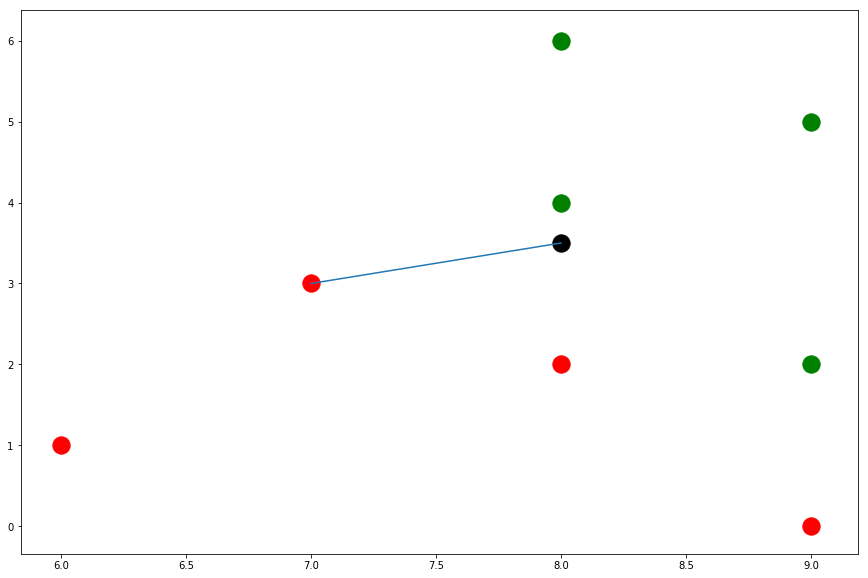
\includegraphics[width=\linewidth]{nn3.png}
                        \captionof{figure}{Bestimmen des zweiten Abstands}
                        \label{fig:nn3}
                    \end{minipage}
                    \hspace*{.1\linewidth}
                    \begin{minipage}[b]{.4\linewidth}
                        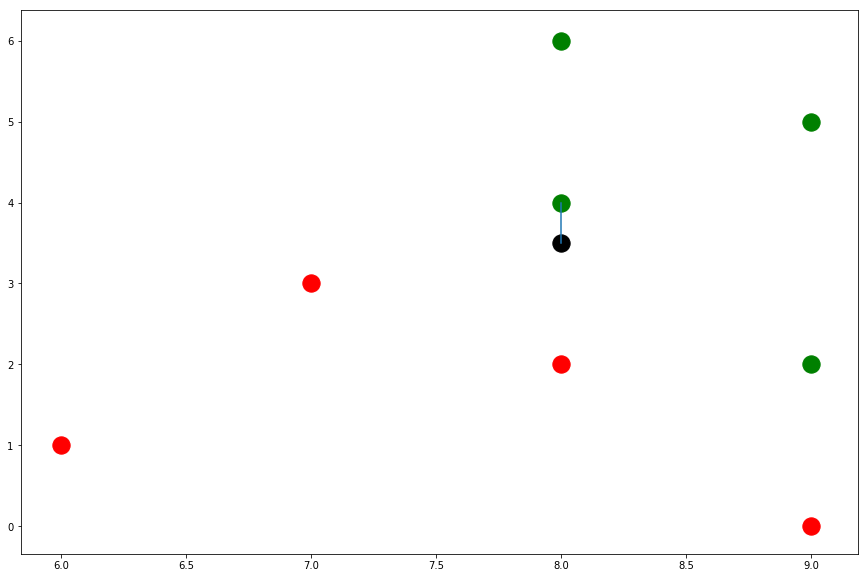
\includegraphics[width=\linewidth]{nn5.png}
                        \captionof{figure}{Bestimmen des $n$-ten Abstands}
                        \label{fig:nn5}
                    \end{minipage}
                \end{Figure}        
                
                        
              %  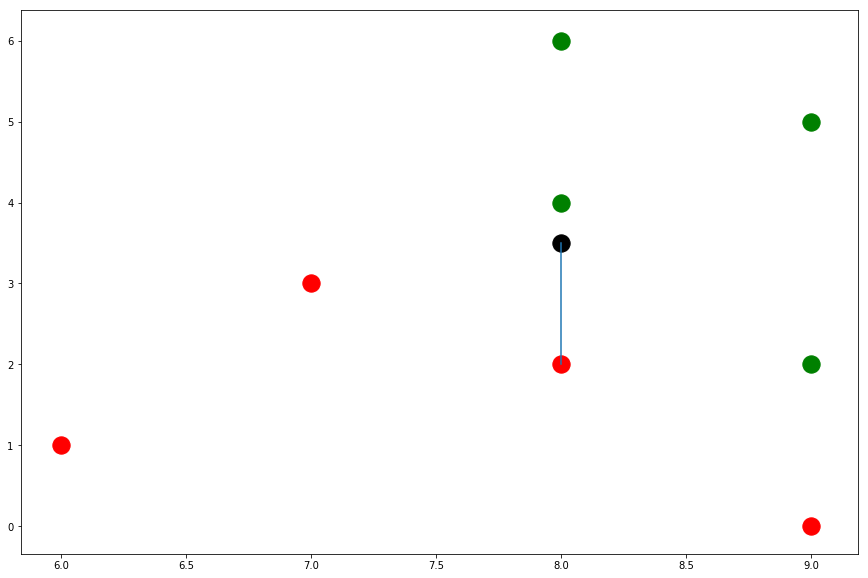
\includegraphics[width=\linewidth]{nn4.png}
               % \captionof{figure}{} % nicht sicher ob diese Grafik gebraucht wird

                  Der gefundene Wert der \emph{argmin\{\}} Funktion verändert sich nicht mehr, nachdem die minimale Distanz ermittelt wurde. Nach Durchlauf aller $n$ Trainingsdaten kann die \emph{argmin\{\}}-Funktion dadurch mit Sicherheit den kleinsten Wert zurückliefern.\par
                   
               	\begin{wrapfigure}{r}{6cm}
                       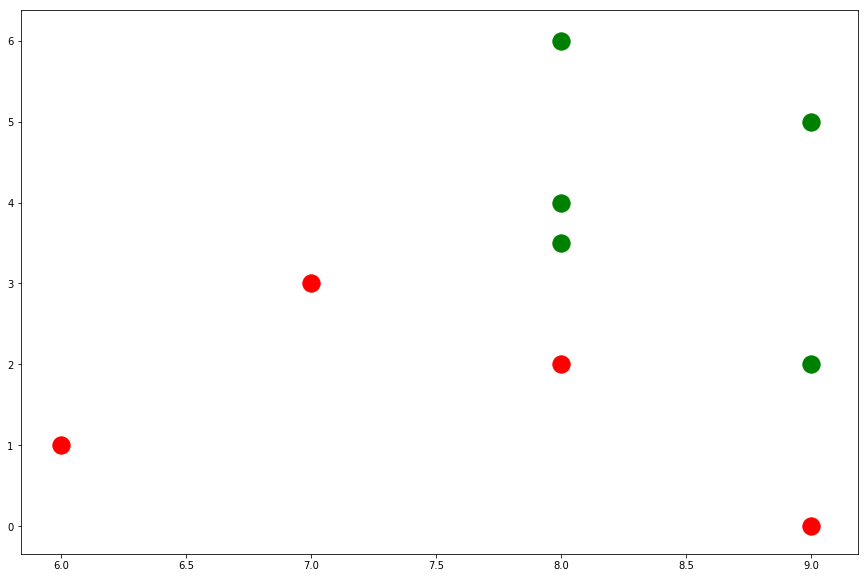
\includegraphics[scale=0.2]{nn6.png}
                        \captionof{figure}{Nach Durchlauf des Algorithmus}
                        \label{fig:nn6}
                \end{wrapfigure}
                
                Im letzten Schritt kann die Klasse des neuen Punktes gesetzt werden, wie in Abb. \ref{fig:nn5} zu sehen, gehört der nächste Nachbar zur grünen Klasse. Daraus kann man schließen, dass der schwarze Punkt aufgrund seiner Ähnlichkeit zum grünen Punkt auch zur selben Klasse gehört.\par
                        
            \subsection{Kritik an der      Nearest-Neighbour Methode}
                Das \emph{nearest Neighbour} Verfahren ist ein mächtiges Werkzeug zum Klassifizieren von Daten, da der Algorithmus selbst anhand nicht linear separable Mengen eine Zuordnung treffen kann.\cite{ertel2016} Wenn das Lernverfahren jedoch mit dem bereits behandelten \emph{Perzeptron} aus Kapitel 4 verglichen wird, fällt auf, dass der \emph{nearest Neighbour} Algorithmus im $\mathbb{R}^2$ keine lineare Trennlinie bzw. im Raum des $\mathbb{R}^n$ keine trennende Hyperfläche erzeugt. Dies ist insoweit ungünstig, da anhand dieser Trennfunktion für jeden weiteren zu klassifizierenden Punkt weniger Aufwand betrieben werden muss, die zugehörige Klasse zu ermitteln.\cite{ertel2016}\par
                Weiterer Kritikpunkt des \emph{nearest Neighbour} ist, dass im Falle von statistischen Ausreißern in den Trainingsdaten Datenpunkte möglicherweise falsch zugeordnet werden. Ein statistischer Ausreißer bedeutet im Falle des \emph{nearest Neighbour} Algorithmus, dass sich innerhalb der Trainingsdaten ein oder mehr falsch klassifizierte Datenpunkte befinden. Dieses Problem besteht selbst dann, wenn in unmittelbarer Nähe zum Betrachtungspunkt weitere korrekt klassifizierte Trainingsdaten zur Verfügung stehen. Das liegt daran, dass bei dieser Variante des \emph{nearest Neighbours} nur der erste nächste Nachbarn zur Klassifizierung betrachtet wird.\cite{ertel2016}\par

                         
               % Schaubild Beispiel Nearest Neighbour mit Ausreißer.
                In Abbildung \ref{fig:errnn1} wird diese Ausgangssituation mit fehlerhaften Trainingsdaten beschrieben, um zu verdeutlichen, wie ein einzelner Irrtum das gesamte Verfahren verfälschen kann. \par 
                \begin{Figure}
                    \begin{minipage}[b]{.4\linewidth}
                        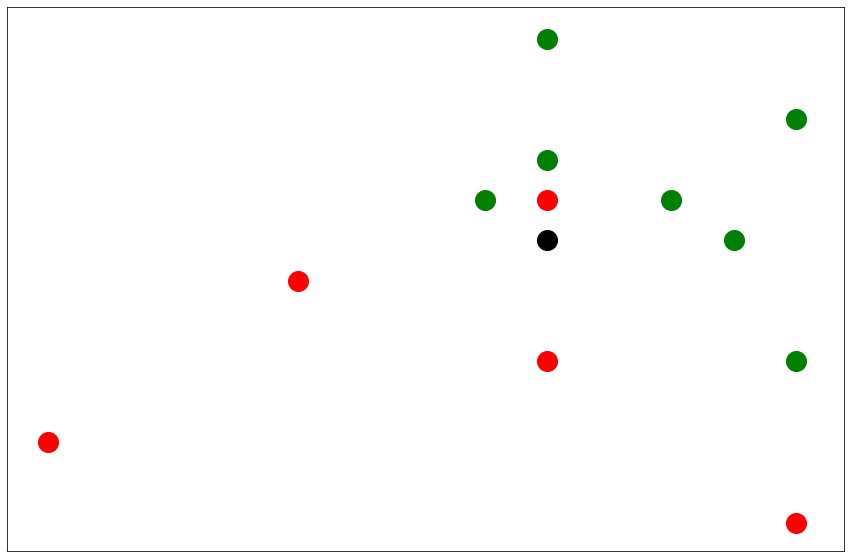
\includegraphics[width=\linewidth]{errnn1.png}
                        \captionof{figure}{Ausgangssituation mit Ausreißer}
                        \label{fig:errnn1}
                    \end{minipage}
                    \hspace*{.1\linewidth}
                    \begin{minipage}[b]{.4\linewidth}
                        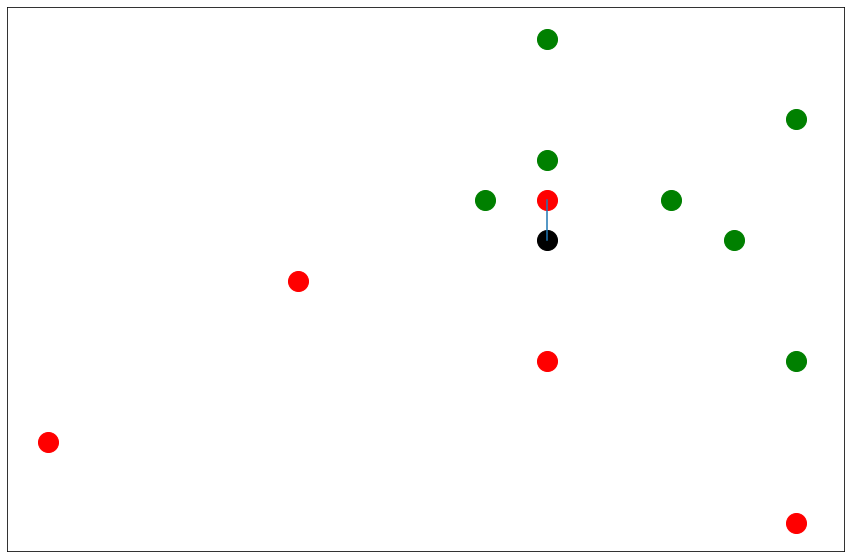
\includegraphics[width=\linewidth]{errnn2.png}
                        \captionof{figure}{Bestimmen des minimalen Abstands}
                        \label{fig:errnn2}
                    \end{minipage}
                \end{Figure}

                \begin{Figure}
                    \centering
                    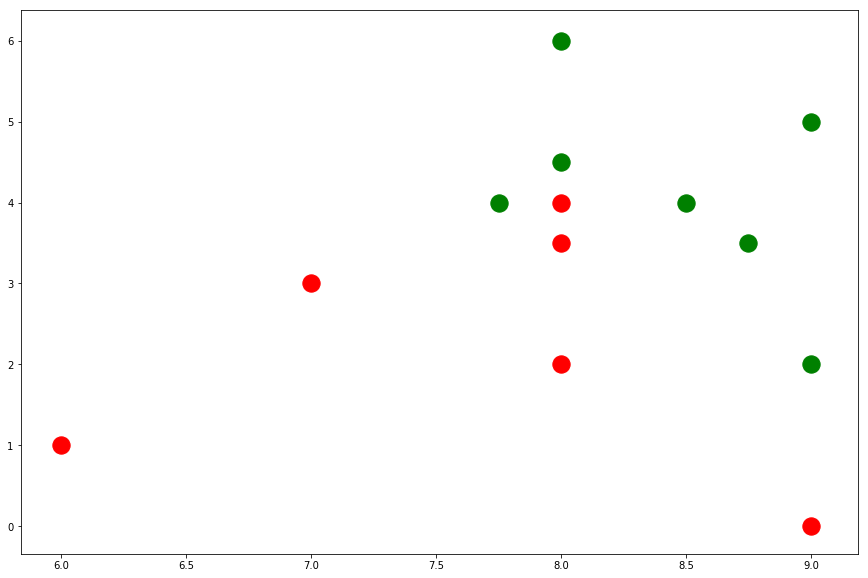
\includegraphics[scale=0.2]{errnn3.png}
                    \captionof{figure}{Fehlklassifizierung nach Durchlauf}
                    \label{fig:errnn3}  
                \end{Figure}
                
                  Man erkennt, dass sich ein rot klassifizierter Punkt in unmittelbarer Nähe von mindestens drei Punkten der grünen Klasse befindet. % die nochmal verdeutlichen soll, wie ein einziger statistischer Ausreißer bei dem \emph{nearest Neighbour} Verfahren fehlerhafte Klassifizierungen verursacht.\par 
                                %In Abbildung 16 sieht man ...
                   Auf diese Daten wird nun analog zu Kapitel \ref{subsec:nnalgo} das Lernverfahren des \emph{nearest Neighbour} angewendet.\par
                   %suchanker
                
                Es werden erneut alle Datenpunkte auf minimalen Abstand zum (schwarzen) Ausgangspunkt überprüft. Die \emph{argmin\{\}}-Funktion liefert für diesen Fall den statistischen Ausreißer als Referenzpunkt zurück (siehe Abb. \ref{fig:errnn2}). Abschließend erfolgt die Klassifizierung zur Klasse rot(siehe Abb. \ref{fig:errnn3}).\par
                Demnach ist es dem System nicht möglich zu wissen, ob ein Punkt aus den Trainingsdaten fehlerhaft oder korrekt ist und kann auch für diesen Fall nicht auf andere verfügbare Daten zurückgreifen. Für dieses Problem ist die \emph{nearest Neighbour} Methode, wie sie in diesem Kapitel beschrieben ist, nicht mächtig genug.
                         
        \section{k-nearest Neighbour Methode}
            Ist eine Variante des \emph{nearest Neighbour}. Bei der Verwendung des \emph{k-nearest Neighbour} Algorithmus wird statt einem nächsten Nachbarn eine k-große Gruppe an nächsten Nachbarn betrachtet. Die Entscheidung zu welcher Klasse ein neuer Datenpunkt gehören soll, erfolgt durch einen Mehrheitsentscheid innerhalb dieser ermittelten k-nächsten Nachbarn.\cite{ertel2016}\par
            Es werden die gleichen Bezeichner für den Algorithmus verwendet, die auch für den \emph{nearest Neighbour} angewandt wurden und um die Variable $V$ erweitert.\par $V$ bezeichnet die k-nächsten Nachbarn von $s$ innerhalb der Trainingsdaten.
        	\newpage
                           
            \subsection{k-nearest Neighbour Algorithmus}
                Der Algorithmus ist wie folgt definiert:\par
                \begin{algorithm}[H]
                    \KwData{$M_+,M_-,s \in \mathbb{R}^n$}
                    \KwResult{Klassifikation von $s$}
                    $V= $\{k-nächste Nachbarn von $s$\}\;
                    \If{$|M_+ \cap V| > |M_- \cap V| $}{
                        \KwRet{+}\;
                    }
                    \eIf{$|M_+ \cap V| < |M_- \cap V| $}{
                        \KwRet{-}\;
                    }  
                    {
                        \KwRet{Random(+,-)}\;
                    }
                           
                    \caption{k-Nearest Neighbour Algorithm nach \cite[S.209]{ertel2016}}
                \end{algorithm}\par
                
                
                Im Folgenden wird ein Beispiel für den \emph{k-nearest Neighbour} behandelt. Es stehen in Abb. 19 rot und grün klassifizierte Punkte als Trainingsdaten zur Verfügung und zu bestimmen ist die Klasse des schwarzen Punktes.\par  
                % Schaubilder
                \begin{Figure}
                    \begin{minipage}[b]{.25\linewidth}
                        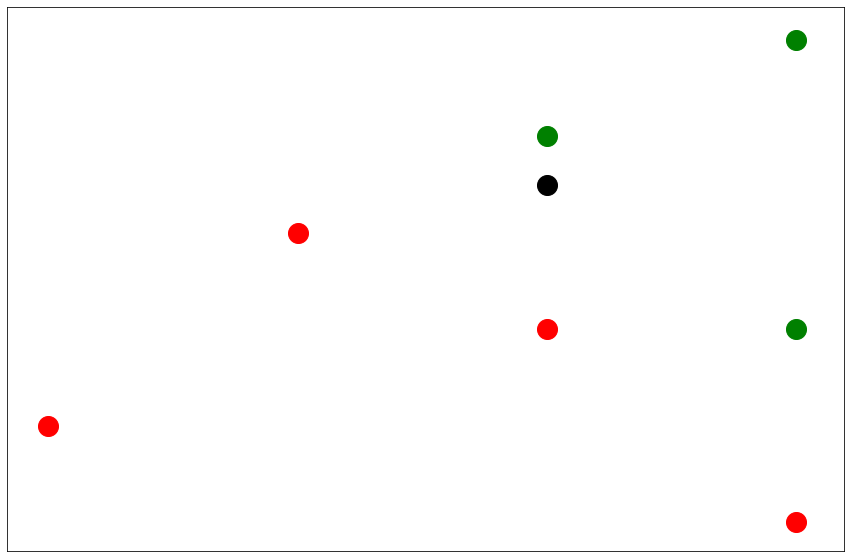
\includegraphics[width=\linewidth]{knn1_neu.png}
                        \captionof{figure}{Ausgangssituation}
                        \label{fig:knn1}
                    \end{minipage}
                    \hspace{.1\linewidth}
                    \begin{minipage}[b]{.25\linewidth}
                        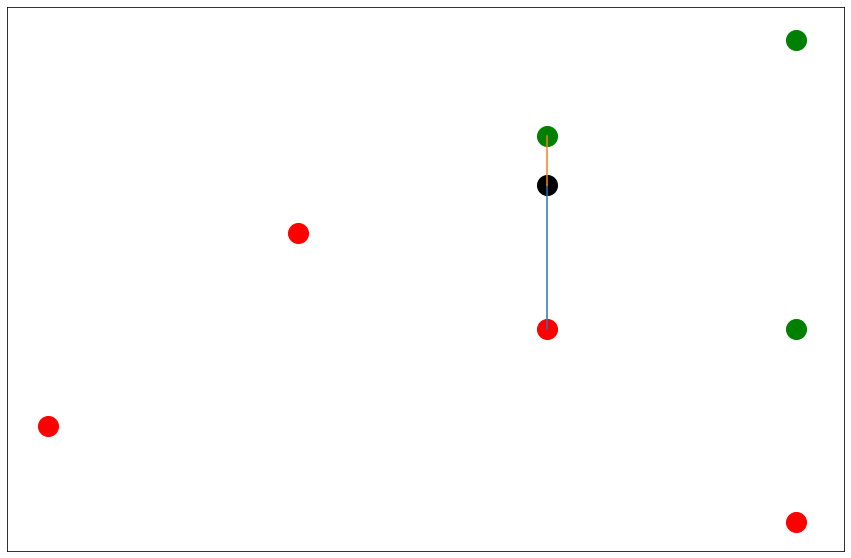
\includegraphics[width=\linewidth]{knn3.png}
                        \captionof{figure}{Fall $k=2$}
                        \label{fig:knn3}
                    \end{minipage}
                    \hspace*{.1\linewidth}
                    \begin{minipage}[b]{.25\linewidth}
                        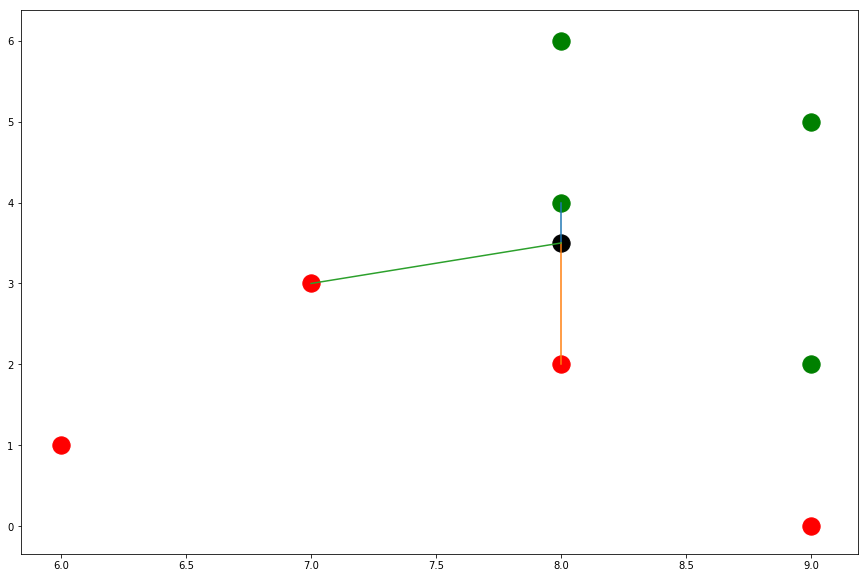
\includegraphics[width=\linewidth]{knn4.png}
                        \captionof{figure}{Fall $k=3$}
                        \label{fig:knn4}
                    \end{minipage}
                \end{Figure}
                
                Für den Fall $k=1$, also die Betrachtung nur eines einzelnen nächsten Nachbars, kann auf das Ergebnis aus Kapitel \ref{subsec:nnalgo} verwiesen werden.\par  
              	              
          %      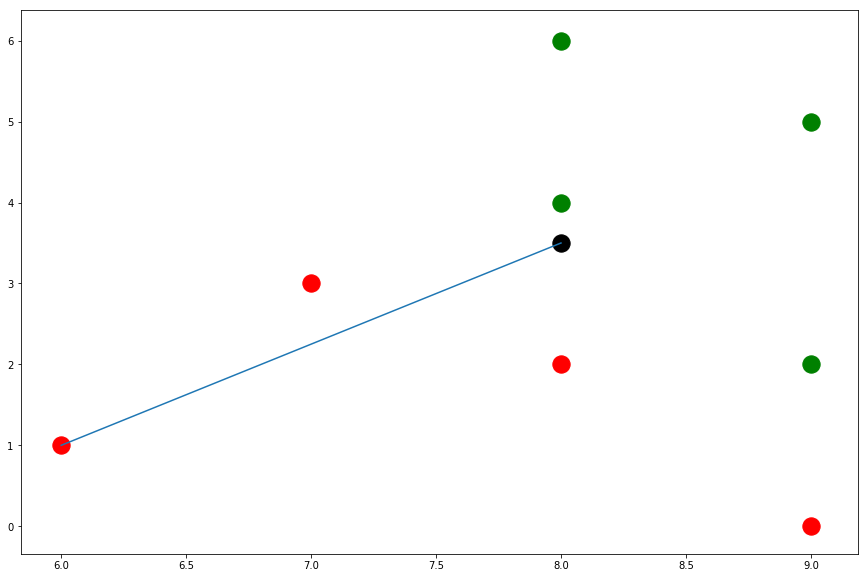
\includegraphics[width=\linewidth]{nn2.png} Werden beide nicht benötigt
           %     \captionof{figure}{}
                         
          %      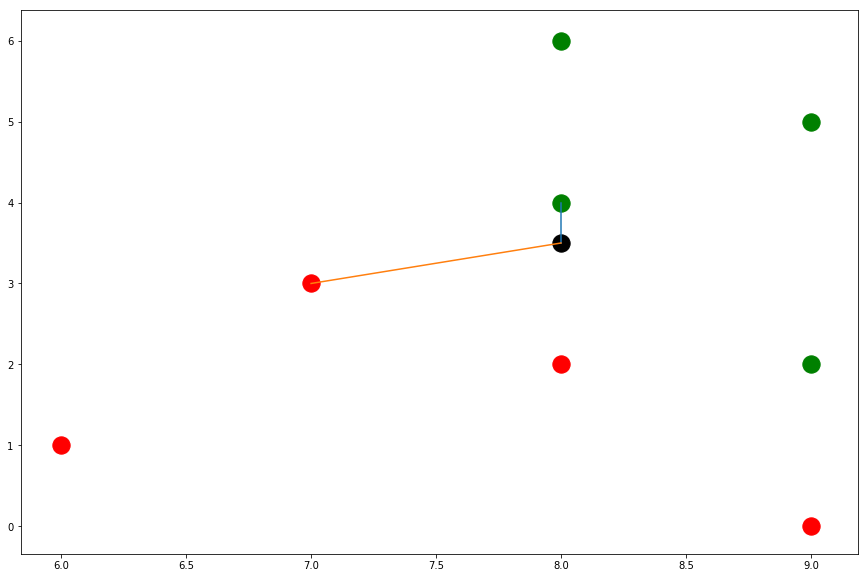
\includegraphics[width=\linewidth]{knn2_b.png}
          %      \captionof{figure}{}
                        
                
              Der Fall $k=2$ kann aus Abb. \ref{fig:knn3} entnommen werden. Hierbei wird die Menge betrachteter nächster Nachbarn auf zwei erhöht und führt dazu, dass bei Anwendung des Algorithmus die zwei kleinsten Abstände über die Abstandsfunktion zu ermitteln sind. Die Variable $V$ enthält nach Bestimmen aller Distanzen jeweils einen Punkt aus der roten und grünen Klasse.

                $$
                    V=\{\text{rot,grün}\}
                $$ 
                Als Nächstes werden die Schnittmengen von $V$ mit den jeweiligen Klassen ausgewertet.\par 
                Es folgt also:
                $$
                    |V \cap \text{Rot}| = 1 \text{ und } | V \cap \text{Grün} | = 1
                $$
                Für die Klasse des schwarzen Punktes bedeutet dies, dass seine Klasse zufällig aus der Menge \{Rot, Grün\} ausgewählt werden muss.     
                \par
            	In Abb. \ref{fig:knn4} wird die Anzahl nächster Nachbarn mit Stimmrecht erneut um eins erhöht. Die Verbindungen zwischen dem schwarzen Punkt und allen anderen zeigen, welche der Punkte im Merkmalsraum die kleinsten Abstände aufweisen. Dadurch enthält $V=$ \{rot, rot, grün\} und daraus folgt demnach für die Schnittmengen:
                $$
                    |V \cap \text{Rot} | = 2 \text{ und } | V \cap \text{Grün} | = 1
                $$
            	Für die Zugehörigkeit des schwarzen Punktes ergibt sich somit eine Klassifizierung in Richtung der roten Klasse.
            	
            	Auf die gleiche Weise kann $k \rightarrow n$ weitergeführt werden.
                        
            \subsection{Anwendung bei mehr als zwei Klassen}
                Es ist ebenfalls möglich den \emph{k-nearest Neighbour} nicht nur für zwei Klassen anzuwenden, sondern auch auf endlich viele Klassen zu erweitern. Hier steht man jedoch vor der Herausforderung, falls die Anzahl Klassen ansteigt, wächst im gleichen Zug die Anzahl der benötigten Trainingsdaten stark an.\cite{ertel2016}\par
                Noch weiter verschärft wird dieses Szenario, wenn nicht genug Trainingsdaten oder Speicherressourcen zur Verfügung stehen. 
                %problematisch wird die Situation wenn man nicht genug Trainingsdaten zur Verfügung stehen oder Speicherressourcen nicht ausreichen.
                Steigt die Anzahl der Klassen weiter, ist eine diskrete Klassifikation nicht mehr ideal und eine stetige Abbildungsfunktion ist für die Anwendung zweckmäßiger.\cite{ertel2016}
                \par
                Auf die Betrachtung der Laufzeit wird in Kapitel \ref{sec:laufzeit} eingegangen.
                
            \subsection{Kritik an der k-nearest Neighbour Methode}
            \label{subsec:kritikknn}
                Analog gilt ebenfalls für die \emph{k-nearest Neighbour} Methode, dass die Anwendung des Algorithmus allein keine Trennebene erzeugen kann.
                Andererseits kann festgehalten werden, dass der Algorithmus eine schwächere Anfälligkeit gegenüber statistischen Ausreißern aufweist. Grund dafür ist die Betrachtung einer größeren Stichprobe der Trainingsdaten.\par
                        
                Ein weiterer Kritikpunkt lautet, dass bei wachsendem k, also bei Betrachtung eine größer werdenden Gruppe nächster Nachbarn, die Anzahl weiter entfernter Nachbarn einen nicht unwesentlichen Einfluss auf den Mehrheitsentscheid und somit auf die Klassifizierung eines Datenpunktes haben. Dies steht im Widerspruch zu dem zentralen Ähnlichkeitsbegriff (Vgl. Kapitel 5.1), welcher geringe Abstände als Ähnlichkeitsmaß definierte.\par
                Eine Möglichkeit zur Verbesserung ist laut Wolfgang Ertel, die Stimmen der k-nächsten Nachbarn mit Gewichten zu versehen. Die Stimmgewichte der nächsten Nachbarn sollen mit steigendem Abstand zum zu klassifizierenden Punkt quadratisch abnehmen, um dadurch weniger Einfluss ausüben zu können.\cite{ertel2016}\par

                        
                Die Bestimmung der Stimmgewichte $w$ ist wie folgt definiert:\par
                $x$ ist der zu klassifizierende Punkt und $x_i$ ist der i-te nächste Nachbar von $x$.
                $$
                    x,x_i \in \mathbb{R}^n
                $$
                $$
                    w_i:=\frac{1}{1+\alpha d(x,x_i)^2} \text{ \footnotesize\cite[S.212]{ertel2016}}
                $$
                \par
                $\alpha$ ist ein Konstante und bestimmt, wie schnell Gewichte mit größer werdendem Abstand zum Ausgangspunkt abnehmen sollen.\cite{ertel2016} Anhand dieser Formel erkennt man, dass mit wachsendem Abstand der Einfluss bzw. das Stimmgewicht weit entfernter Punkte asymptotisch gegen null geht und ist somit ein zielführender Lösungsansatz.\cite{ertel2016}\par

        \section{Voronoi-Diagramme}
            Im Kapitel \ref{subsec:kritikknn} (Titel: Kritik an der \emph{nearest Neighbour} Methode) wurde bereits erwähnt, dass der \emph{nearest Neighbour} Algorithmus im Vergleich zum \emph{Perzeptron} keine (lineare) Trennebene erzeugen kann. Es ist jedoch möglich durch Hinzunahme eines weiteren Verfahrens nicht nur eine Trennung vorzunehmen, sondern auch eine wesentlich komplexere Trennebene aus den gegebenen Trainingsdaten zu schaffen, um so die benötigte Rechenzeit zur Klassifizierung zu vermindern.\cite{ertel2016}
            Wie bereits bei den \emph{Eager Learning} Algorithmen erklärt wurde, benötigt die Bestimmung dieser Abbildungsfunktion den Großteil der Rechenzeit. Ein Verfahren aus der Kategorie des \emph{Lazy Learnings} wird auf diese Weise um ein Verfahren, dass man dem \emph{Eager Learning} zuordnen würde, erweitert.\par Die Bestimmung der Trennebene ist daher mit einem Zusatzaufwand verbunden, jedoch wird der Merkmalsraum um eine nützliche Eigenschaft ergänzt. Denn mithilfe des \emph{Voronoi-Diagramms} wird um jeden Punkt ein beliebig komplexes Polygon erzeugt. Innerhalb jedes Polygons gilt, dass der nächste Nachbar genau jener Punkt ist, um den das Polygon anfangs gebildet wurde.\cite{ertel2016} \par
            
            Auf die konkrete Bestimmung eines \emph{Voronoi-Diagramms} für eine endliche Datenmenge wird nur beschränkt eingegangen, da lediglich das Ergebnis für unsere Anwendung von Interesse ist. %Vorallem, weil es den Rahmen der Ausarbeitung sprengen würde.
                        
        \subsection{Voronoi-Diagramm Beispiel}
        Als Beispiel wird die folgende Ausgangssituation (siehe Abb. \ref{fig:v1}) betrachtet. Zwei Klassen als grüne Plus und rote Minus gekennzeichnet dienen als Menge von Trainingsdaten. Für diese Menge soll nun als Nächstes das zugehörige \emph{Voronoi-Diagramm} genauer untersucht werden. \par
        Auf den ersten Blick erkennt man, dass die Trennung in keinem Falle durch eine lineare Gerade erzeugt werden kann, da sich links und rechts von Punkten der grünen Klasse jeweils Punkte der roten Klasse befinden. Dadurch kann man die Aussage treffen, dass die vorgegebene Trainingsdatenmenge nicht Teil der linear separablen Mengen ist und demnach zu keiner Lösung bei Verwendung der \emph{Perzeptron}-Lernregel führen würden.
            \begin{Figure}
                \begin{minipage}[b]{.4\linewidth}
                    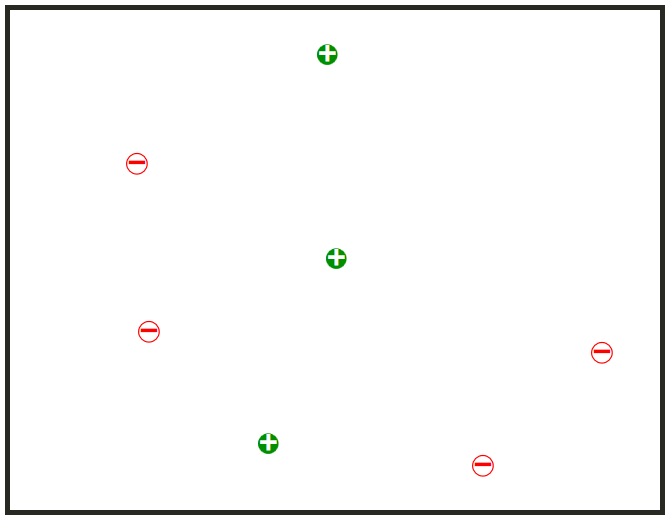
\includegraphics[width=\linewidth]{vor1.png}
                \captionof{figure}{Zu klassifizierende Punkte}
                \label{fig:v1}   
                \end{minipage}
                \hspace*{.1\linewidth}
                \begin{minipage}[b]{.4\linewidth}
                    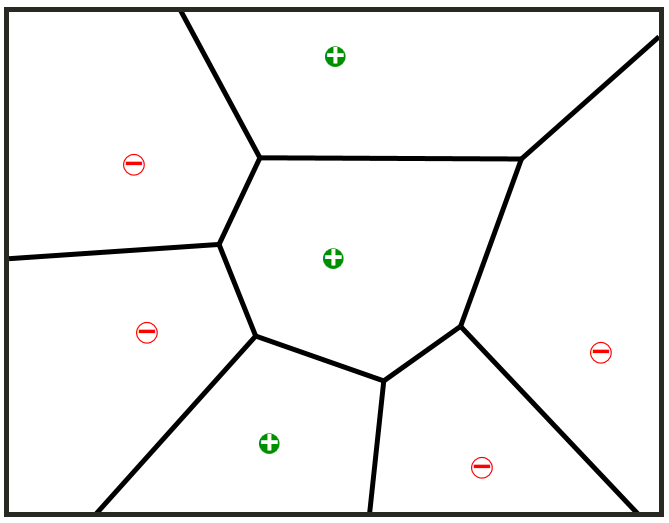
\includegraphics[width=\linewidth]{vor2.png}
                    \captionof{figure}{Eintragen der Polygone}
                    \label{fig:v2}
                \end{minipage}
            \end{Figure}

            In Abbildung \ref{fig:v2} fällt auf, dass unabhängig von der Klasse eines Punktes eine Gerade orthogonal auf der Mitte einer imaginären Verbindung zwischen dem betrachteten Punkt und seinen umliegenden Nachbarn liegt. Diese Geraden bilden, wenn für alle näheren Nachbarn eingezeichnet, das Polygon in welchem er sich befindet. Dies lässt sich auf die Eigenschaft des \emph{Voronoi-Diagramms} zurückführen, dass innerhalb des Polygons jeder Punkt näher am zentralen Punkt gelegen ist, als an jedem anderen Punkt innerhalb des Merkmalsraums.
            
            \begin{Figure}
                \centering
                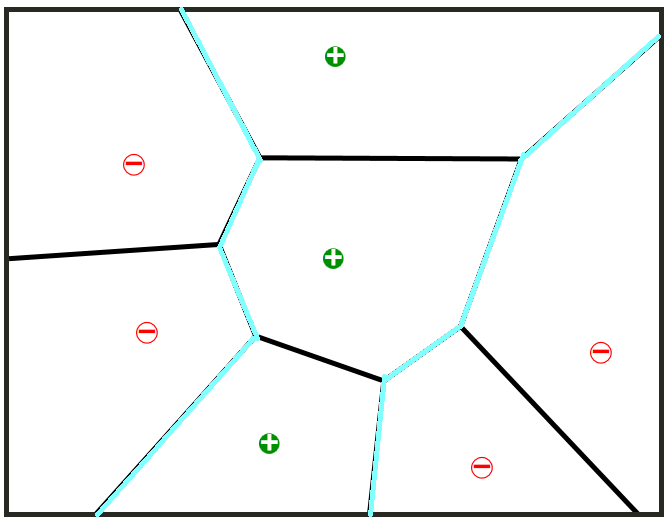
\includegraphics[width=.4\linewidth]{vor3.png}
                \captionof{figure}{Trennung von zwei Klassen
                \label{fig:v3}
                }
            \end{Figure}

            Nachdem das \emph{Voronoi-Diagramm} für eine Menge von Trainingsdaten ermitteln wurde, kann eine Trennebene eingezeichnet werden (siehe Abb. \ref{fig:v3}). Die Trennung hat die Eigenschaft, dass sich innerhalb Trennebene nur Datenpunkte einer Klasse befinden. Wird anschließend der Versuch unternommen eine Klassifizierung durchzuführen, kann man dies anhand der Trennlinie mit geringem Aufwand unternehmen, indem geprüft auf welcher Seite der Trennung sich der zu bestimmende Punkt befindet. Infolgedessen wird die Berechnungszeit gestrichen, die man ohne \emph{Voronoi-Diagramm} für das Ermitteln aller Abstände zum Betrachtungspunkt genutzt hätte.\par
            Die Diskussion in welchem Verhältnis die Berechnung des \emph{Voronoi-Diagrammms} zu der Zeit, die man für jede Ausführung einspart, steht, würde den Rahmen dieser Ausarbeitung übersteigen und wird nicht weiter ausgeführt.\par
            Man kann folglich mithilfe dieses Beispiels den Beweis erbringen, dass die \emph{nearest Neighbour} Methode ein mächtigeres Klassifizierungsverfahren ist als das \emph{Perzpetron}.
            
            % Nachdem das Voronoi-Diagramm für eine Menge von Trainingsdaten ermitteln wurde, kann eine Trennebene eingezeichnet werden (siehe Abb. \ref{fig:v3}). Die Trennung hat die Eigenschaft, dass sich innerhalb Trennebene nur Datenpunkte einer Klasse befinden. Wird anschließend der Versuch unternommen eine Klassifizierung durchzuführen, kann man dies anhand der Trennlinie mit geringem Aufwand unternehmen. Für das Beispiel bedeutet das...
                         
        \section{Laufzeiten der nearest-Neighbour Methoden}
        \label{sec:laufzeit}
            Laut Wolfgang Ertel: \glqq Gibt es kein [maschinelles] Lernverfahren, dass so schnell lernt”\grqq \cite[S. 213]{ertel2016}, wie die \emph{nearest Neighbour} Methode, da in diesem Fall nur Daten gesichert werden müssen.\par
            Wie der Rechenaufwand für beide vorgestellten Methoden aussieht wird im Folgenden gezeigt.
                        
            \subsection{Laufzeit nearest-Neighbour Algorithmus}
                Bei der Betrachtung des \emph{nearest Neighbour} Algorithmus fällt auf, dass jeder enthaltene Punkt der Trainingsdaten auf eine minimale Distanz zum Betrachtungspunkt untersucht werden muss. Somit gilt für die Laufzeit:
                $$
                    \mathcal{O}(n)
                $$   
            
            \subsection{Laufzeit        k-nearest-Neighbour Algorithmus}
                Der \emph{k-nearest Neighbour} Algorithmus hat ähnlich, wie der \emph{nearest Neighbour}, eine Grundlaufzeit von $n$, jedoch entsteht bei der Iteration über alle ermittelten nächsten Nachbarn ein zusätzlicher Rechenaufwand der Größe $k$. Dadurch ergibt sich für die Laufzeit:
                $$
                    \mathcal{O}(n+k)
                $$
                Bei den \emph{nearest Neighbour} Methoden gibt es keine Fallunterscheidung in bessere oder schlechtere Ausgangssituationen, da bei keiner Konstellation der Trainingsdaten Unterschiede im Ablauf entstehen. \par
                Nicht außer Acht gelassen werden darf die Tatsache, dass mit $n$ nur die Anzahl verfügbarer Trainingsdaten gemeint ist und nicht verwechselt werden darf mit der Anzahl Dimensionen aus denen ein Punkt aus dem Merkmalsraum geformt ist.  

    %\end{multicols}

    \newpage

    \bibliography{literatur}
    \bibliographystyle{alpha}
\end{document}
